% Docummentation: 
% - https://www.latex-project.org/help/documentation/
% - https://docs.w3cub.com/latex/
% - https://tex.stackexchange.com/questions/455993/formatting-sql-code
%   https://www.overleaf.com/learn/latex/Code_listing#Code_styles_and_colours

%--------------------------------------------------------------------------------
%-----------------------------------   TODO   ----------------------------------
%--------------------------------------------------------------------------------
%Add in dcummentation 
% - class description - basic PySimpleGUI class
% - applicatin can become crossplatform in the future (check how installers work)
%
%Needed functions:
% - Save and read (persistent) configuration - https://www.pysimplegui.org/en/latest/cookbook/#recipe-the-demo-browser Recipe - Save and Load Program Settings ( https://www.pysimplegui.org/en/latest/#user-settings-api )
% - Data quarantine for bad inputs - store data that did not go through 
% validation and let user correct it [preferably also provide reason why it was quarantined] 
% - Data export to csv
%
%Optional functions:
% - Data statistics (records in each table, firstdate-lastdate, data quality)
% - Change GUI theme: add selectable list with themes, store it in config #DONE
% - synopsis for functions
% - built in manual
% - error handling
% - Localization - Language versions
% - logs (easy-ish): logfile.append(date, event)
% - fix in place table editting
% - allow user to remove data
% - (loose idea) VERY optional: create database programatically: 
% 	- dump database creation script into sql file
%	- create dummy Finances.sqlite wherever user wants
%	- use script as database initialisation
% - automatically deduce the encoding GetDataFromCSV
% - add tresholds to graph (automatic based on average, user specified)
% - add predicted spending next month (requires: to ProductSummary and 
%		ProductType Sumary add columns mean[median?] cost (Amount/Bought Times),
%	  AverageDailyCost (Amount/(lastbought-firstbought))
% - change used database technology to secure data, centralize and allow simultaneous users

\documentclass[a4paper,10pt, twoside]{report}

\usepackage{polski}         % Polish diacretic signs
\usepackage[utf8]{inputenc} % required for international characters
\usepackage{hyperref}       % urls and hyperlinks
\usepackage{xurl}           % break urls
\usepackage{microtype}      % improve justification
\usepackage{enumitem}       % compact lists
\usepackage{graphicx}       % Include graphics
\usepackage{wrapfig}        % wrap text aroung graphics
\usepackage{fancyhdr}       % Customize page layout
\usepackage{index}          % Create an index
\usepackage{setspace}       % Spacing
\usepackage{float}          % Forcing figure placement
\usepackage{tabularray}     % Tables with wrapping
\usepackage{xcolor,listings}% Code listings
\usepackage{textcomp}       % Code listings
\usepackage{color}          % Code listings
\usepackage{nameref}        % Reference chapter, section, etc. by name
\usepackage{afterpage}
\usepackage{tcolorbox}      % Colored boxes for inline Code

\makeindex
\graphicspath{ {./} }       %Was ./figures/ changed so i can peek in VS Code


% Code listings
\definecolor{codegreen}{rgb}{0,0.6,0}
\definecolor{codegray}{rgb}{0.5,0.5,0.5}
\definecolor{codepurple}{HTML}{C42043}
\definecolor{backcolour}{HTML}{F2F2F2}
\definecolor{bookColor}{cmyk}{0,0,0,0.90}  
\color{bookColor}

\lstset{upquote=true}

\lstdefinestyle{mystyle}{
    backgroundcolor=\color{backcolour},   
    commentstyle=\color{codegreen},
    keywordstyle=\color{codepurple},
    numberstyle=\numberstyle,
    stringstyle=\color{codepurple},
    basicstyle=\footnotesize\ttfamily,
    breakatwhitespace=false,
    breaklines=true,
    captionpos=b,
    keepspaces=true,
    numbers=left,
    numbersep=10pt,
    showspaces=false,
    showstringspaces=false,
    showtabs=false,
}
\lstset{style=mystyle}

% Code listings
\newcommand\numberstyle[1]{%
    \footnotesize
    \color{codegray}%
    \ttfamily
    \ifnum#1<10 0\fi#1 |%
}

\renewcommand{\lstlistlistingname}{Listingi}

% ------------------------------ Custom Commands ------------------------------
% Usage: \command\{text}  
\newcommand{\customstyletitle}[1]{\Huge{\textbf{#1}}}
\newcommand{\customstylechapter}[1]{\large{\textit{#1}}}
\newcommand{\customstylesection}[1]{\textbf{\textit{#1}}}
\newcommand{\customstylesidenote}[1]{\Small{\textbf{#1}}}
\newcommand{\customstyletable}[1]{\footnotesize{\textbf{#1}}}
\newcommand{\customstyletablecentered}[1]{\footnotesize\centering{\textbf{#1}}}
\newcommand{\customstyleindivisible}[1]{
    \begin{minipage}{\textwidth}
        {#1}
    \end{minipage}
}

\lstnewenvironment{SQLlisting}[2][]%
  {\noindent\minipage{\linewidth}\medskip
   {#2}
   \smallskip
   \lstset{basicstyle=\ttfamily\footnotesize,
            frame=single,
            language=SQL,
            deletekeywords={IDENTITY},
            %deletekeywords={[2]INT},
            morekeywords={clustered},
            framesep=8pt,
            xleftmargin=40pt,
            framexleftmargin=40pt,
            frame=tb,
            framerule=0pt,
            caption=#1}}
  {\endminipage}

  % spacer
\newcommand{\HRule}{\rule{\linewidth}{0.5mm}} % horizontal lines

\newtcbox{\inlinecode}{on line, boxrule=0pt, boxsep=0pt, top=2pt, left=2pt, bottom=2pt, right=2pt, colback=gray!15, colframe=white, fontupper={\ttfamily \footnotesize}}

% --------------------------- documment starts here ---------------------------

% environment
\begin{document}

% Define pagestyle
% [REQUIREMENT] 23. Przypisy dolne, stopki (nr stron), nagłówki...
\pagestyle{fancy}
\fancyhf{}          %clears default headers and footers
\renewcommand{\headrulewidth}{2pt}
\renewcommand{\footrulewidth}{1pt}

\fancypagestyle{mychapterpage}{%
    %\fancyhead[LE]{\leftmark}
    %\fancyhead[RO]{\rightmark}
    \fancyfoot[RO,LE]{\thepage}
    \renewcommand{\headrulewidth}{2pt}
    \renewcommand{\footrulewidth}{1pt}
}


% https://texblog.org/2013/09/16/multiple-page-styles-with-fancyhdr/
%Redefine chapter by adding fancy as the chapter title page page-style
\makeatletter
    \let\stdchapter\chapter
    \renewcommand*\chapter{%
    \@ifstar{\starchapter}{\@dblarg\nostarchapter}}
    \newcommand*\starchapter[1]{%
        \stdchapter*{#1}
        \thispagestyle{mychapterpage}
        \fancyfoot[RO,LE]{\thepage}
        \markboth{\MakeUppercase{#1}}{}
    }
    \def\nostarchapter[#1]#2{%
        \stdchapter[{#1}]{#2}
        \thispagestyle{mychapterpage}
        \fancyfoot[RO,LE]{\thepage}
    }
\makeatother


% [REQUIREMENT] 1. Strona tytułowa
\begin{titlepage}
	%---Headings------------------------------------------	
	\begin{center}
    \begin{onehalfspace}
    \textsc{\LARGE{WYŻSZA SZKOŁA TECHNOLOGII INFORMATYCZNYCH W KATOWICACH}}\\
    \end{onehalfspace}
    \textsc{\large{WYDZIAŁ INFORMATYKI}}\\
	\textsc{\large{KIERUNEK: INFORMATYKA}}\\
    \end{center}
    
    %---Author--------------------------------------------
	\begin{flushleft}
    \textsc{Nowak Marcin}\\[0cm]
    \textsc{Nr Albumu 08255}\\[0cm]
    \textsc{Studia niestacjonarne}\\[0cm]
    \end{flushleft}
	
    %---Title---------------------------------------------
	\begin{center}
    \HRule\\[0.4cm]
	{\customstyletitle{Projekt i implementacja aplikacji wspomagającej zarządzanie budżetem domowym}}\\[0.4cm] 
    \HRule\\[1.5cm]
    \end{center}
	
    %---Description----------------------------------------
	\begin{flushright}
        \textsc{Przedmiot: Projekt Systemu Informatycznego}\\[0cm]
        \textsc{pod kierunkiem}\\[0cm]
        \textsc{mgr. Jacek Żywczok}\\[0cm]
        \textsc{W roku akademickim 2022/23}\\[0cm]
    \end{flushright}
 
	%---Date & logo---------------------------------------
	\vfill                  % Position the date lower
	\begin{center}
    {Katowice 2022}\\	    % \today
	
\includegraphics[width=0.2\textwidth]{figures/WSTI-logo.jpg}\\[1cm]
	\end{center}
\end{titlepage}

%TODO: fix, this moves formatting 
\null\newpage %TODO: fix, this moves formatting \addtocounter{page}{-1}

% [REQUIREMENT] 2. Spis treści
\renewcommand*\contentsname{Spis treści}
\tableofcontents                    % prints automatical table of contents

% ---------------------------------- Content ----------------------------------

% [REQUIREMENT] 3. Wprowadzenie do tematyki projektu
\chapter{\customstylechapter{Wprowadzenie do tematyki projektu}}
{Finanse są dziedziną nauki ekonomicznej któa zajmuje się rozporządzaniem 
pieniędzmi \cite{wiki_ekonomia}. Nauka ta w podobnym zakresie a różnej skali 
dotyczy państw, przedsiębiorstw jak i zwykłych obywateli - w efekcie jest to 
dziedzina o stosunkowo prostych podstawach jednak niesamowicie skomplikowana w 
każdym zakresie w którym można ją zagłębić. Wiedza z zakresu finansów staje się 
szczególnie przydatna gdy na rynku panuje trudna sytuacja ekonomiczna, w takich 
warunkach nierzadko decyduje ona o jakości oraz stanie życia poszczególnych 
osób fizycznych, rentowności przedsiębiorstw czy stabilności państw. W przypadku
 państw i firma przeważnie budżetem zarządzają dedykowane osoby lub też całe 
zespoły, posiadające ekspercką wiedzę w tej dziedzinie. Jednak osoby 
zarządzające budżetem domowym najczęściej dysponują wyłacznie nabytym 
doświadczeniem, rzadko jeśi wogóle wspomagając się jakimikolwiek narzędziami 
które ułatwiałyby to zadanie.}
%
% [REQUIREMENT] 4. Zamierzony cel projektu
\chapter{\customstylechapter{Zamierzony cel projektu}}
{Celem projektu jest utworzenie modułu analitycznego aplikacji któa ułatwi 
zarządzanie budżetem domowym dostarczając użytkownikowi narzędzia do analizy 
wpływów i wydatków, wizualizacji trendów oraz automatycznie kategoryzujące 
wpływy i wydatki.} 

{Docelowymi odbiorcami aplikacji są użytkownicy domowi, możliwe że w miarę 
rozwoju w późniejszych fazach projektu także średnie lub małe przedsiębiorstwa. 
Użytkownik po wprowadzeniu danych uzyska dostęp do możliwie czytelnego obrazu 
sytuacji finansowej co uwidoczni trendy wydatków i przychodów, pozwoli bardziej
 świadomie podejmować dalsze decyzje finansowe, planować budżet a także łatwo
 identyfikować obszary które wymagają usprawnień. W efekcie uwidocznione przez
 aplikację informacje i wyciągnięte z nich wnioski ułatwią użytkownikowi poprawę
 sytuacji finansowej swojego domostwa poprzez bardziej efektywne zarządzanie
 budżetem.}
%
% [REQUIREMENT] 5. Wstępne założenia i uwarunkowania, w których 
% projekt będzie powstawał  -----------------------
\chapter{\customstylechapter{Wstępne założenia i uwarunkowania}}
\section{\customstylesection{Założenia}}
{Z uwagi na specyfikę tematyki potencjalnymi odbiorcami aplikacji będą osoby 
w niewielkim lub średnim stopniu zaznajomione z obsługą komputera. Największy
wpływ na projekt i rozwój graficznego interfejsu użytkownika oraz kierunek
 rozwoju aplikacji będzie miała łatwość obsługi. W efekcie aplikacja powinna
 być możliwie prosta, mieć przejrzysty, minimalistyczny interfejs dzięki 
czemu użytkownik nie zostanie przytłoczony mnogością dostępnych funkcji.}

{Początkowo użytkownik będzie wprowadzał dane do aplikacji samodzielnie poprzez 
dedykowany interfejs. Aplikacja zadba o jakość danych przyjmując jednak 
oznaczając i pomijając dane błędne, niepełne lub niepewne które zaprezentuje w 
dedykowanej zakładce gdzie użytkownik będzie mieć możliwość ich poprawy. 
Użytkownik będzie w stanie wybrać zestaw predefiniowanych typów i kategorii 
wydatkó lub utworzyć i edytować własne. Aplikacja udostępni predefiniowane 
wizualizacje, wliczając możliwość wizualizacji określonego przez użytkownika 
produktu lub całej kategorii produktów. We wstępnej wersji aplikacji interfejs
będzie statyczny, podobnie jak konfiguracja, która przechowywana będzie w pliku.}

\section{\customstylesection{Uwarunkowania}}
{Jest to projekt edukacyjny którego celem jest dostarczenie minimalnego
 opłacalnego produktu \cite{MVP}, swego rodzaju prototypu, na tym etapie funkcje
 dodatkowe zostaną pominięte ze względu na ograniczony czas produkcji, zakres
 umiejętności technicznych autora. Bliski termin oddania wyklucza bardziej
 zaawansowane funkcje, a znajomość technologii będzie budowana w trakcie jego
 rozwoju co wpłynie między innymi na ograniczenia systemowe. Aplikacja będzie
 także z zasady obsługiwać wyłącznie pojedynczego użytkownika, a dane przez
 niego wprowadzone będa przechowywane wyłącznie lokalnie. Pominięte zostanie
 także automatyczne pobieranie danych z interfejsów innych aplikacji lub w
 formie ekstrakcji danych ze skanowanych dokumentów czy kodów EAN lub QR
 produktów. Aplikacja nie będzie także udostępniać żadnego rodzaju interfejsu 
programistycznego (API). Założono że na tym etapie interfejs aplikacji będzie statyczny bez
 możliwości zmiany przez użytkownika.}

%Removed due to overspill:
% W momencie zakończenia projektu wszystkie dane
% użytkownika przechowywane będą w pojedynczym miejscu, w przyszłości może 
% jednak zajść potrzeba rozdzielenia danych w aplikacji od konfiguracji 
% użytkownika.

% [REQUIREMENT] 6. Założone ograniczenia (ramy czasowe, umiejętności) 
% i możliwość ewaluacji projektu
%[TODO] Shorten title to FIX overspill in table of contents 
\chapter{\customstylechapter{Założone ograniczenia i możliwości ewaluacji projektu}}
{W miarę możliwości standard danych w aplikacji dopasowany zostanie do wiodącego
 globalnego standardu danych w obrębie tej samej tematyki. Typy obiektów będzie
 można grupować na kilku poziomach aby ułatwić użytkownikowi zarządzanie danymi
 i uprościć wizualizacje. Dla zaawansowanych użytkowników może okazać się 
przydatna możliwość definiowania i zapisywania własnych wizualizacji i raportów 
statystycznych - wymagać to będzie jednak implementacji dedykowanego modułu. 
Kolejnym obecnie pominiętym aspektem jest zabudowanie reguł przeprowadzających 
dogłębną analizę statystyczną danych które otwierają dalsze możliwości rozwoju 
oprogramowania. Aplikacja dostarczana będzie użytkownikom w formie spakowanej w
archiwum skompilowanej pełnej wersji, jeśli zajdzie taka potrzeba i pojawi się 
możliwość stworzony zostanie także instalator. Możliwe że w aplikacji utworzony 
zostanie panel administracyjny prezentujący użytkownikowi dane statystyczne 
obrazujące ilość, zakres i jakość danych a także sugerujące kolejny krok ich 
usprawnienia.}

{Funkcje importu i eksportu danych ze standardowych formatów będą przydatne dla 
użytkownika podczas korzystania z projektu, wymaga określenia odpowiedniego 
formatu i standardu plików co może zająć sporo czasu dlatego zostały uznane za 
dodatkowe przez co możliwe że nie zostaną wdrożone w początkowej fazie projektu.}

{Obrane podejście pozwoli na rozwój aplikacji w różnych kiernkach, zależnie od 
opinii użytkowników. Aplikacja może zmienić model z aplikacji lokalnej która 
wspiera pojedynczego użytkownika na centralny obsługujących wielu użytkowników 
zdalnie. Ujednolicony interfejs umożliwia także powstanie potencjalnej wersji 
mobilnej co otworzy nowe możliwości wprowadzania danych oraz interakcji 
użytkownika z aplikacją.}
% [REQUIREMENT] 7. Chronologiczny plan pracy (ujecie przyjetego modelu 
% projektowania i faz projektowania)
\chapter{\customstylechapter{Plan pracy}}
{W toku prac stworzona zostanie lista zadań do zrealizowania, do określenia ich 
priorytetu posłuży metoda MoSCoW \cite{MOSCOW} lub Matryca Eisenhowera 
\cite{MatrycaEisenhowera}. Przewidywany plan pracy nad projektem prezentuje się następująco:
\setitemize{noitemsep,topsep=0pt,parsep=0pt,partopsep=0pt}
\begin{enumerate}
    \item Spis założeń w dokumentacji wstępnej
    \begin{itemize}
        \item Założenia wstępne
        \item Spis wymagań każdego typu
        \item Przegląd rynku pod kątem dostępnych rozwiązań
        \item Określenie metodologii pracy
        \item Dokumentacja modelowania
        \item Dokumentacja uruchomieniowa projektu
        \item Przeprowadzone testy
        \item Instrukcja obsługi dla użytkownika
        \item Retrospekcja
    \end{itemize}
    \item Modelowanie 
    \begin{itemize}
        \item Utworzenie słownika modelowanej domeny
        \item Określenie wymaganych kontenerów
        \item Określenie wymaganych encji i atrybutów
        \item Określenie wymaganych ograniczeń danych
        \item Modelowanie powiazań encji
    \end{itemize}
    \item Wybór technologii
    \begin{itemize}
        \item Wspierane systemy i wersje
        \item Wybór języka
        \item Biblioteki interfejsu użytkownika
        \item Sposób przechowywania danych
        \item Instalator, aktualizacja i utrzymanie 
    \end{itemize}
    \item Wstępne wdrożenie
    \begin{itemize}
        \item Utworzenie bazy danych
        \item Utworzenie podstawowych struktur bazy danych - tabele
        \item Wypełnienie danymi testowymi
        \item Utworzenie złożonych struktur bazy danych - widoki
        \item Projekt interfejsu użytkownika
        \item Szkielet interfejsu użytkownika
        \item Połączenie interfejsu z bazą danych
        \item Projekt podstawowych wizualizacji
        \item Iteracyjna uzupełnienie interfejsu i bazy o dodatkowe funkcje
        \item Usprawnienia i refaktoryzacja
    \end{itemize}
    \item Testy rozwiązania
    \begin{itemize}
        \item Utworzenie danych testowych
        \item Określenie spodziewanych wyników
        \item Porównanie wyników oczekiwanych z otrzymanymi
    \end{itemize}
    \item Iteracyjne usprawnienia projektu i uzupełnianie dokumentacji
    \item Retrospekcja
    \begin{itemize}
        \item Przydatność gotowej aplikacji
        \item Wady i zalety podejścia
        \item Sprawność rozwiązań
        \item Sprawność technologii
        \item Spis wniosków
    \end{itemize}
\end{enumerate}
}

% [REQUIREMENT] 9. Wymagania funkcjonalne (szczegółowey wykaz wszystkich funkcji 
% oprogramowania) jakie funkcjonalności oprogramowania chcemy dostarczyć, można 
% nie zdążyć z dostarczeniem części, lub dopisać dodatkowe dodane w trakcie
\chapter{\customstylechapter{Wymagania funkcjonalne}} 
\label{Wymagania funkcjonalne}
{Zestawienie funkcji które powinien spełniać program, wraz z informacją któe 
z nich zostały spełnione. Nagłówki z powodu objętości zostały skrócone, legenda:}

{PRIO - Priorytet w jednej z kategorii MOSCOW \cite{MOSCOW}}

{IMPL - Oznaczenie czy funkcję wdrożono}

%[TODO]: try tabularray as suggested
% Wrapping as per: https://stackoverflow.com/questions/790932/how-to-wrap-text-in-latex-tables
\begin{table}[h]
    \footnotesize
    \begin{tabular}{|p{0.2\linewidth}|p{0.07\linewidth}|p{0.07\linewidth}|p{0.52\linewidth}|}  % | draws verical line
    % \usepackage{booktabs} provides different line thicknesses
    % \toprule, \midrule, \bottomrule
    \hline                  % Draw horizontal line
        
    % & Defines the breaks in the table 
    \customstyletable{Funkcja} & \customstyletablecentered{PRIO} & \customstyletablecentered{IMPL}& \customstyletable{Opis} \\
    \hline
    {Plik konfiguracji} & {M} & {TAK} & {Osobny plik konfiguracyjny}\\
    \hline
    {Dodawanie danych} & {M} & {-} & {Dodawanie danych}\\
    \hline
    {Podsumowanie wydatków} & {M} & {TAK} & {Okresowe podsumowanie wydatków}\\
    \hline
    {Podsumowanie przychodów} & {M} & {TAK} & {Okresowe podsumowanie przychodów}\\
    \hline
    {Statystyki typów} & {C} & {TAK} & {Statystyki wydatków na dany typ produktu}\\
    \hline
    {Statystyki produktów} & {C} & {TAK} & {Statystyki wydatków na dany produkt}\\
    \hline
    {Bilans okresowy} & {M} & {TAK} & {Okresowy bilnas zysków i strat}\\
    \hline
    {Definiowanie produktów} & {M} & {TAK} & {Definiowanie produktów}\\
    \hline
    {Definiowanie przychodów} & {M} & {TAK} & {Definiowanie przychodów}\\
    \hline
    {Definiowanie typów produktów} & {M} & {TAK} & {Definiowanie typów produktów}\\
    \hline
    {Definiowanie typów przychodów} & {C} & {NIE} & {Definiowanie typów przychodów}\\
    \hline
    {Panel konfiguracyjny} & {S} & {TAK} & {Osobny panel konfiguracyjny}\\
    \hline
    {Rejestr zdarzeń} & {S} & {NIE} & {Logi z działania aplikacji}\\
    \hline
    {Dostęp zdalny} & {C} & {NIE} & {Dostęp do zdalnych baz danych}\\
    \hline
    {Import danych} & {C} & {TAK} & {Import danych w standardowym formacie}\\
    \hline
    {Walidacja danych} & {C} & {-} & {Potwierdzenie jakości danych}\\
    \hline
    {Eksport danych} & {C} & {-} & {Eksport danych do standardowego formatu}\\
    \hline
    {Instalator} & {C} & {NIE} & {Prosty instalator aplikacji}\\
    \hline
    {Trendy} & {W} & {NIE} & {Predykcja trendów wydatkó i wpływów}\\
    \hline
    {Porady} & {W} & {NIE} & {Porady dla użytkownika dotyczące usprawnień budżetu}\\
    \hline
    {Wiele użytkowników} & {W} & {NIE} & {Wsparcie dla wielu użytkowników jednocześnie}\\
    \hline
    {Personalizacja interfejsu} & {W} & {TAK} & {Personalizacja interfejsu użytkownika}\\
    \hline
    {Aktualizacje} & {W} & {NIE} & {Automatyczne sprawdzanie wersji i aktualizacja}\\
    \hline
    \end{tabular}
    \caption{Wymagania funkcjonalne}
\end{table}

% [REQUIREMENT] 10. Wymagania niefunkcjonalne 
\chapter{\customstylechapter{Wymagania niefunkcjonalne}}
% [REQUIREMENT] 10.1. Sprzętowe (w różnych wariantach, w tym dostęp do 
% koniecznych lub alternatywnych nośników danych i peryferiów)
\section{\customstylesection{Sprzętowe wymagania niefunkcjonalne}}
\begin{itemize}
    \item Pamięć 50MB dowolnego typu
    \item Pamięć RAM 4GB (wliczajac system)
    \item Urządzenia peryferyjne: klawiatura, mysz komputerowa
    \item Dowolne urządzenie wyświetlające
\end{itemize}
% [REQUIREMENT] 10.2. Systemowe (systemy operacyjne, zainstalowane środowiska, 
% platformy, pakiety, biblioteki, sterowniki)
\section{\customstylesection{Systemowe wymagania niefunkcjonalne}}
% Wzory: https://www.microsoft.com/pl-pl/windows/Windows-10-specifications
% https://examsoft.com/resources/examplify-minimum-system-requirements/
% https://softwareengineering.stackexchange.com/questions/86863/how-are-minimum-system-requirements-determined
{System Operacyjny Windows 1, Python 3 z biblioteką matplotlib, PySimpleGUI - 
instalowane poleceniami:}

\inlinecode{python -m pip install -U matplotlib}

\inlinecode{python -m pip install -U pysimplegui}

% [REQUIREMENT] 10.3. Organizacyjne (np. organizacja pracy z systemem, warunki 
% poprawnej pracy przy większej liczbie użytkownikó, stanowisk, obciążeniu sieci,
% konieczność zapewnienia realnego czasu dostępu itd.itp.)
\section{\customstylesection{Organizacyjne wymagania niefunkcjonalne}}
{Projekt aplikacji obejmuje interakcje z pojedynczym użytkownikiem w danym 
momencie, każdy z użytkowników będzie korzystał z własnej instancji bazy 
danych aplikacji która bedzie przechowywana w dowolnej dogodnej określonej 
przez użytkownika pamięci lokalnej określonej w pliku konfiguracyjnym, a także 
zdalnej jeśli wdrożona zostanie funkcja dostępu zdalnego. Aplikacja 
wstępnie nie będzie wymagała stałego dostępu do sieci, jednak w przyszłości 
jej rozwój może zmienić to wymaganie - wymagać wtedy będzie krótkich okresów 
dostępu do sieci. Dostęp do danych będzie wymagany w krótkich okresach zapisu 
danych z pamięci podręcznej aplikacji do bazy oraz odpytania bazy o dane. 
Aplikacja powinna być wykorzystywana na systemach zabezpieczonych przed dostępem
 osób niepowołanych.}

% [REQUIREMENT] 11. Wymagania dotyczące danych (wykaz tabel, relacji, 
% typy i rozmiary pól z uzasadnieniem, inne rodzaje danych w tym logi, hasła)
\chapter{\customstylechapter{Wymagania danych}}
{W tej sekcji spisano wymagania wstępne, jak w każdym projekcie wymagania 
zmieniały się wraz z jego rozwojem w trakcie modelowania i 
wdrażania. Aktualny reprezentatywny stan danych w aplikacji z wyróżnieniem 
wszystkich warstw opisuje rozdział \nameref{Opisy metod}.}

{Użytkownik będzie wprowadzał dane do aplikacji ręcznie lub za pomocą interfejsu
importującego dane w formacie CSV (Comma Separated Values) \cite{CSV}. Dane 
wprowadzone przez użytkownika po walidacji trafią odpowiedniej tabeli w bazie 
danych, natomiast te któe walidacji nie przejdą do zbioru tymczasowego w którym 
użytkownik będzie je mógł poprawić - po przejściu prawidłowo walidacji trafią 
do zbioru docelowego. Wszystkie dane wprowadzone przez użytkownika będą 
traktowane jako ciągi znaków a następnie rzutowane na typy odpowiadające 
docelowym polom w bazie danych do których zostaną przekazane. Wymagania 
danych w bazie oraz aplikacji podzielono na poszczególne sekcje poniżej.}

\section{\customstylesection{Baza danych}}
{Aplikacja wymaga sposobu na trwałe składowanie danych wprowadzonych przez 
użytkownika. W tym celu wraz z aplikacją każdy użytkownik otrzyma dedykowaną 
lokalną instancję bazy danych SQLite \cite{SQLite} do własnego użytku. Za 
wyborem tej technologii przemawiają niewielkie wymagania przestrzeni pamięci 
trwałej jakie zajmuje oraz w miarę kompletne wsparcie standardowego języka 
zapytań SQL \cite{SQL}.}

{Baza powinna zawierać tabele do przechowywania danych o przychodach, rachunkach
 i wydatkach oraz wszelkie dane pomocnicze wspomagające normalizację danych. 
Powinna zawierać także widoki wspomagające pracę z danymi obliczające w miarę 
możliwości automatycznie dane analityczne wykorzystywane później w aplikacji. 
Aby zachować spójność danych i raportów dane wprowadzane do bazy powinny być 
odpowiednio walidowane, jednak aby zadbać o ich kompletność użytkownik powinien
mieć możliwość świadomie wprowadzić dane które wymagają poprawy do późniejszej 
obróbki.}

{Szczegóły implementacji wraz z kodem opisane zostaną w sekcji \nameref{Baza danych}}

\section{\customstylesection{Kod aplikacji}}
{Python jest językiem elastycznym, dzięki czemu przyjmuje dane w dowolnej 
formie bez definiowania typu, co pozwala odroczyć projekt klas do momentu 
implementacji a nawet refactoringu programu. W języku Python \cite{Python} 
domyślnie wszystkie zmienne są typu Any co pozwala definiować typy zależnie od 
potrzeb w trakcie tworzenia programu. Wszystkie wczytywane z plików dane 
domyślnie przyjmują typ string lub są traktowane jako pojedyncze bajty 
\cite{Python_read-file}. W efekcie dane wprowadzane przez użytkownika przyjmą 
formę ciągów znaków klasy string, po czym w programie zostaną przekazane do 
konstruktorów klas gdzie zostaną rzutowane na odpowiednie do zadań typy i 
zapisane w polach.}

{Aby ułatwić rozwój aplikacji program powinien zapisywać i przyjmować z pliku 
dane konfiguracyjne w formie list ciągów znaków w formacie "opcja" : "wartość" 
które utworzą obiekt słownika, lub w wariancie bardziej zaawansowanym aplikacja 
może przyjmować konfigurację w postaci pliku JSON \cite{JSON}. Rozwiązanie to 
jest na tyle elastycznie że pozwoli dynamicznie definiować dodatkowe 
konfiguracji w trakcie powstawania projektu - aplikacja zaczyta konfigurację z 
pliku i na jej podstawie utworzy słownik, dzięki czemu dodanie nowego parametru 
sprowadzi się do dopisania linijki tektu do pliku.}

{Aplikacja powinna udostępniać użytkownikowi intuicyjne wizualizacje danych 
dostępne przez interfejs użytkownika. Ponieważ jest to projekt edukacyjny 
aplikacja zostanie zaimplementowana w języku Python \cite{Python} którego autor 
chce się nauczyć. Do implementacji interfejsu użytkownika posłuży biblioteka 
PySimpleGUI \cite{PySimpleGUI} która pozwala tworzyć prosty i responsywny, 
niezależny od platformy interfejs o ograniczonych możliwościach. Jest to adapter
 (tak zwany wrapper) który łączy kilka popularnych bibliotek służących do 
tworzenia interfejsu, udostępnia spójny interfejs dzięki czemu warstwę 
prezentacji można budować wykorzystując tablice złożone z udostępnianych jako 
obiekty widżetów. W fazie prototypu interfejsu nie będzie można konfigurować z 
poziomu aplikacji, natomiast niewykluczone że użytkownik będzie w stanie zmienić
 podstawowe ustawienia edytując dostarczony plik konfiguracyjny. Szczegóły 
implementacji interfejsu opisano w sekcji 
\nameref{Graficzny interfejs użytkownika}.}

{W samym kodzie aplikacji podstawymi strukturami wizualizacji będą kolekcje 
złożone z dat i wartości typu double. Wizualizacje będą przechowywane w 
słownikach, które na podstawie klucza w formacie string służącego także jako 
nazwa wizualizacji zwrócą wartość w formacie string którą będzie zapytanie do 
konkretnej tabeli w bazie danych. Szczegóły implementacji kodu opisano w sekcji 
\nameref{Logika aplikacji}.}


% [REQUIREMENT] 12. Metody pracy, narzędzia i techniki
\chapter{\customstylechapter{Metody pracy, narzędzia i techniki}}
\section{\customstylesection{Metody pracy}}
{Aby dostarczyć minimalny opłacalny produkt \cite{MVP} aplikacja będzie 
rozwijana poprzez wdrażanie wymaganych funkcji w kolejności wynikającej 
z ich priorytetów. Podczas planowania projektu wykorzystana zostanie 
priorytetyzacja MoSCoW \cite{MOSCOW} która polega na określeniu priorytetu za 
pomocą jednej z poniżej wymienionych kategorii, jak miało to miejsce w sekcji 
\nameref{Wymagania funkcjonalne}:
\begin{figure}[H]           %requires float package
    \caption{MoSCoW}
    \label{fig:MoSCoW}
    \centering  
    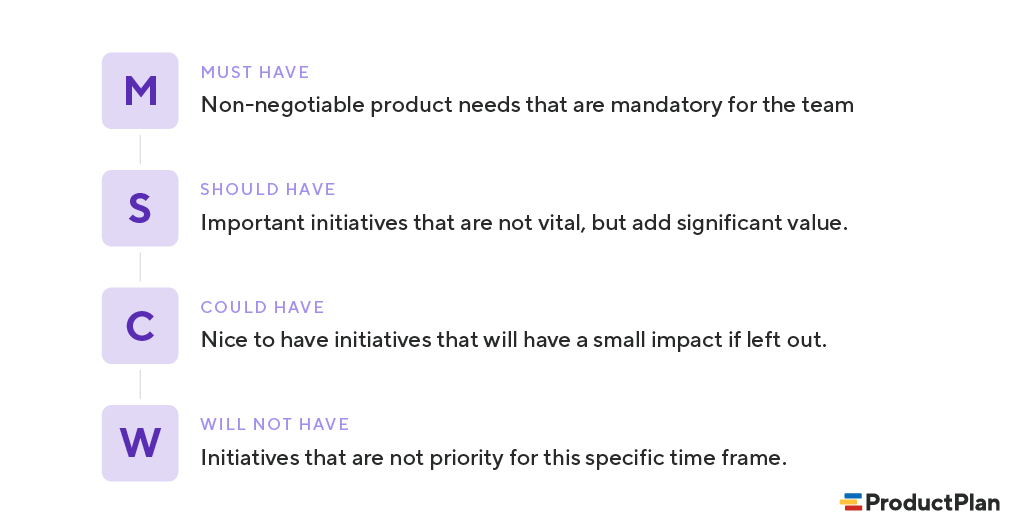
\includegraphics[width=12cm]{figures/MoSCoW-01.png}
\end{figure}
W fazie prototypu zostaną wdrożone wszystkie funkcje wymagane (M), 
natomiast wdrożenie wszelkich pozostałych kategorii zostanie rozpatrzone w fazie
 rozwoju aplikacji. Plan uwzględnia także cykliczne przeglądy priorytetów aby 
 lepiej dopasować aplikację do potrzeb użytkowników i kierunku rozwoju projektu.
 Zadania rozpisane zostaną w metodologii kanban \cite{Kanban}. Zgodnie z 
zasadami LEAN \cite{LEAN} w każdej iteracji kod będzie dodatkowo refaktoryzowany
 i upraszczany, jeśli zajdzie taka potrzeba i uprości to interfejsy funkcji i 
zwiększy czytelność dane zostaną także zebrane w dedykowane klasy.}

\section{\customstylesection{Narzędzia}}
{Podczas projektowania i wdrożenia aplikacji wykorzystane zostaną narzędzia typu
 Open Source oraz komerycjne dostępne nieodpłatnie dla użytkowników 
indywidualnych.}

{Kategoryzacja MoSCoW \cite{MOSCOW} dla poszczególnych funkcji wykonywana będzie
 na zadaniach zarejstrowanych w tablicy kanban, w serwisie serwisu Trello 
\cite{Trello}. Do stworzenia bazy SQLite \cite{SQLite} posłuży aplikacja 
DataGrid \cite{DataGrid}. Aplikacja Visual Studio Code \cite{VSCode} posłuży do
 pisania kodu w Python \cite{Python} oraz dokumentacji w LaTeX \cite{LaTeX}. Do 
rozwoju dokumentacji oraz kodu aplikacji posłuży system kontroli źródła GIT 
\cite{GIT}, a oba kody źródłowe przechowywane będą w osobnych projektach 
\cite[DatabaseShenanigans]{GITBudgeterApp} oraz \cite[budgeter]{GITBudgeterDoc}
 na platformie GitHub \cite{GitHub}.}

\section{\customstylesection{Techniki}}
{W trakcie tworzeznia projektu wykorzystano model przyrostowy 
\cite{Model Przyrostowy} w oparciu o klasyfikację funkcji do wdrożenia metodą 
MoSCoW \cite{MOSCOW}. Ponadto stosowane będą techniki programowania LEAN 
\cite{LEAN} poprawiające czytelność i jakość tworzonego kodu.}

% [REQUIREMENT] 13. Opis głównych klas, metod, obiektów, struktur i algorytmów
% zastosowanych w projekcie (uwzględniając stsosowanie gotowych narzędzi
% obcego autorstwa, w tym open source)
\chapter{\customstylechapter{Opisy metod}} \label{Opisy metod}
\section{\customstylesection{Główne klasy projektu}}
{Projekt składa się z warstw bazy danych oraz graficznego interfejsu aplikacji. 
Baza danych przechowuje dane wprowadzone przez użytkownika w tabelach oraz 
generuje podsumowania i zestawienia w formie widoków. Oba typy obiektów składają
 się na główne klasy projektu. Warstwa graficznego interfejsu użytkownika 
odpowiedzialna jest za interakcję z użytkownikiem oraz interakcję użytkownika z 
bazą - prezentację danych przechowywanych w bazie oraz wizualizacje danych. 
Dodatkowo zbudowano w niej klasy upraszczające interfejs poszczególnych funkcji.}

\section{\customstylesection{Baza danych}}  \label{Baza danych}
{Podczas tworzenia bazy danych przyjęto kilka podstawowych założeń aby utrzymać 
spójną konwencję nazewniczą pól, tabel i widoków. Dzięki niej interfejs bazy 
jest prostszy a pisanie zapytań bardziej intuicyjne co w ogólnym rozrachunku 
powinno ograniczyć nakład pracy wymagany do wdrożenia dodatkowych funkcji.}

\begin{table}[h]
    \footnotesize
    \begin{tabular}{|p{0.2\linewidth}|p{0.73\linewidth}|}  % | draws verical line
    \hline                  % Draw horizontal line
    % & Defines the breaks in the table 
    \customstyletable{Pole} & \customstyletable{Opis} \\
    \hline
    {ID} & {Identyfikator rekordu}\\
    \hline
    {Comment} & {Komentarz użytkownika}\\
    \hline
    {DateTime} & {Znacznik w standardzie daty międzynarodowej ISO 8601 \cite{ISO 8601}}\\
    \hline
    {Amount} & {Koszt, liczba zmiennoprzecinkowa}\\
    \hline
    {Pole specyficzne} & {Główna informacja, różne nazwy w każdej tabeli (Type,Product)}\\
    \hline
    \end{tabular}
    \caption{Konwencja nazewnicza bazy danych }
\end{table}

\begin{figure}[H]           %requires float package
    \caption{Klasy warstwy bazy danych - tabele}
    \label{fig:Klasy warstwy bazy danych - tabele}
    \centering  
    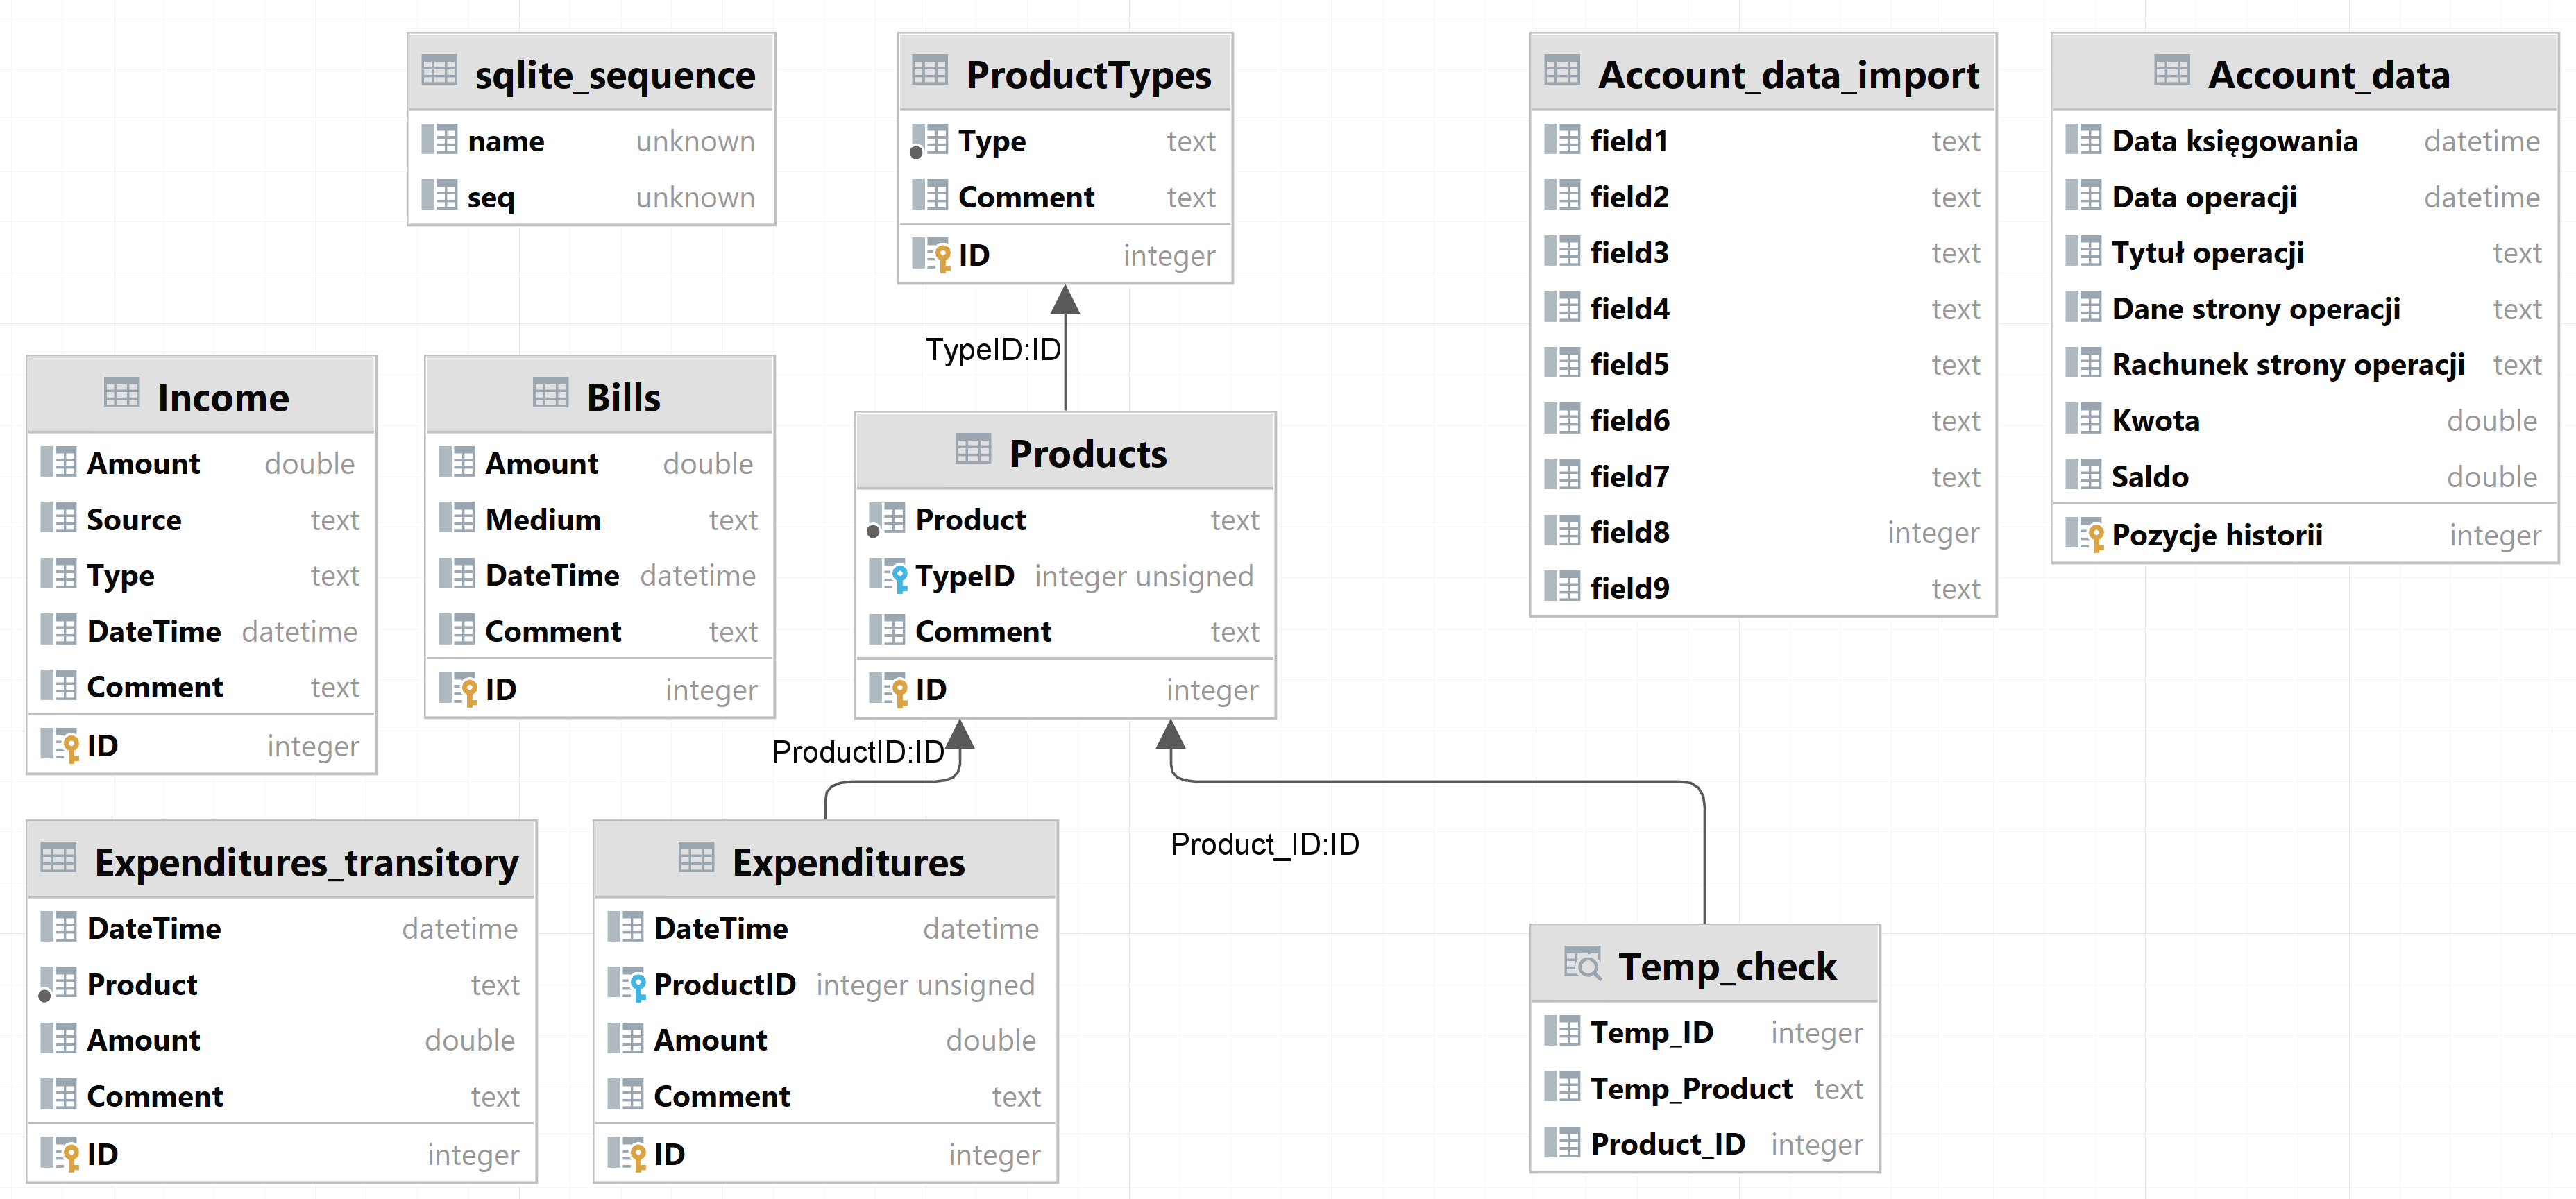
\includegraphics[width=12cm]{figures/Budgeter_Finances-db_Tables_DataGrid.png}
\end{figure}

%-----------------------------TABLES--------------------------------------------
%ADD: Account_data

%[TODO]: Fix - some table span the end of page 
\begin{minipage}{\textwidth}
\begin{lstlisting}[ caption={Tabela ProductTypes},
                    language=SQL,
                    deletekeywords={IDENTITY},
                    deletekeywords={[2]INT},
                    morekeywords={clustered},
                    framesep=8pt,
                    xleftmargin=40pt,
                    framexleftmargin=40pt,
                    frame=tb,
                    framerule=0pt ]
CREATE TABLE [ProductTypes] (
    [ID] 		INTEGER PRIMARY KEY AUTOINCREMENT,
    [Type] 		TEXT 	NOT NULL,
    [Comment] 	TEXT 	DEFAULT NULL
);
\end{lstlisting}
{Tabela ProductTypes zawiera typy produktów zdefiniowane przez użytkownika.}
\end{minipage}

%[TODO] Make function accept 2nd parameter and display caption
%{Tabela ProductTypes zawiera typy produktów zdefiniowane przez użytkownika.}
%\begin{SQLlisting}[{Tabela ProductTypes (v2)}]
%    CREATE TABLE [ProductTypes] (
%        [ID] 		INTEGER PRIMARY KEY AUTOINCREMENT,
%        [Type] 		TEXT 	NOT NULL,
%        [Comment] 	TEXT 	DEFAULT NULL
%    )
%\end{SQLlisting}

\begin{minipage}{\textwidth}
\begin{lstlisting}[ caption={Tabela Products},
    language=SQL,
    deletekeywords={IDENTITY},
    deletekeywords={[2]INT},
    morekeywords={clustered},
    framesep=8pt,
    xleftmargin=40pt,
    framexleftmargin=40pt,
    frame=tb,
    framerule=0pt ]
CREATE TABLE [Products] (
    [ID]        INTEGER PRIMARY KEY AUTOINCREMENT,
    [Product]   TEXT    NOT NULL,
    [TypeID]	INTEGER UNSIGNED, 
    [Comment] 	TEXT    DEFAULT NULL,
FOREIGN KEY([TypeID]) REFERENCES ProductTypes(ID)
);
\end{lstlisting}
{Tabela Products zawiera produkty zdefiniowane przez użytkownika, pole TypeID 
zawiera klucz obcy ID z tabeli ProductTypes.}
\end{minipage}

\begin{minipage}{\textwidth}
\begin{lstlisting}[ caption={Tabela Bills},
    language=SQL,
    deletekeywords={IDENTITY},
    deletekeywords={[2]INT},
    morekeywords={clustered},
    framesep=8pt,
    xleftmargin=40pt,
    framexleftmargin=40pt,
    frame=tb,
    framerule=0pt ]
CREATE TABLE [Bills] (
    [ID]        INTEGER PRIMARY KEY AUTOINCREMENT,
    [Amount]    DOUBLE,
    [Medium]    TEXT,
    [DateTime]  DATETIME,
    [Comment]   TEXT DEFAULT NULL
);
\end{lstlisting}
{Tabela Bills zawiera wydatki stałe wprowadzone przez użytkownika.}
\end{minipage}

\begin{minipage}{\textwidth}
\begin{lstlisting}[ caption={Tabela Income},
    language=SQL,
    deletekeywords={IDENTITY},
    deletekeywords={[2]INT},
    morekeywords={clustered},
    framesep=8pt,
    xleftmargin=40pt,
    framexleftmargin=40pt,
    frame=tb,
    framerule=0pt ]
CREATE TABLE [Income] (
	[ID] 		INTEGER PRIMARY KEY AUTOINCREMENT,
	[Amount]	DOUBLE,
	[Source]	TEXT,
	[Type]		TEXT,
	[DateTime]	DATETIME,
	[Comment]	TEXT DEFAULT NULL
);
\end{lstlisting}
{Tabela Income zawiera przychody wprowadzone przez użytkownika.}
\end{minipage}

\begin{minipage}{\textwidth}
\begin{lstlisting}[ caption={Tabela Expenditures},
    language=SQL,
    deletekeywords={IDENTITY},
    deletekeywords={[2]INT},
    morekeywords={clustered},
    framesep=8pt,
    xleftmargin=40pt,
    framexleftmargin=40pt,
    frame=tb,
    framerule=0pt ]
CREATE TABLE [Expenditures] (
	[ID]	INTEGER,
	[DateTime]	DATETIME,
	[ProductID]	INTEGER UNSIGNED,
	[Amount]	DOUBLE,
	[Comment]	TEXT DEFAULT NULL,
	PRIMARY KEY([ID] AUTOINCREMENT),
	FOREIGN KEY([ProductID]) REFERENCES [Products]([ID])
);
\end{lstlisting}
{Tabela Expenditures zawiera wydatki wprowadzone przez użytkownika.}
\end{minipage}

\begin{minipage}{\textwidth}
\begin{lstlisting}[ caption={Tabela Expenditures\_transitory},
    language=SQL,
    deletekeywords={IDENTITY},
    deletekeywords={[2]INT},
    morekeywords={clustered},
    framesep=8pt,
    xleftmargin=40pt,
    framexleftmargin=40pt,
    frame=tb,
    framerule=0pt ]
CREATE TABLE [Expenditures_transitory] (
	[ID]	INTEGER,
	[DateTime]	DATETIME,
	[ProductID]	INTEGER UNSIGNED,
	[Amount]	DOUBLE,
	[Comment]	TEXT DEFAULT NULL,
	PRIMARY KEY([ID] AUTOINCREMENT),
	FOREIGN KEY([ProductID]) REFERENCES [Products]([ID])
);
\end{lstlisting}
{Tabela Expenditures\_transitory jest tabelą tymczasową, przechowuje wydatki 
wprowadzone przez użytkownika które nie przeszły walidacji. Użytkownik poprawia 
je po czym prawidłowe dane są przenoszone do tabeli Expenditures i  usuwane z 
Expenditures\_transitory.}
\end{minipage}


%------------------------------VIEWS--------------------------------------------
%[TODO]: Add Ledger_comparison, MonthlyCharge

\begin{figure}[H]           %requires float package
    \caption{Klasy warstwy bazy danych - widoki}
    \label{fig:Klasy warstwy bazy danych - widoki}
    \centering  
    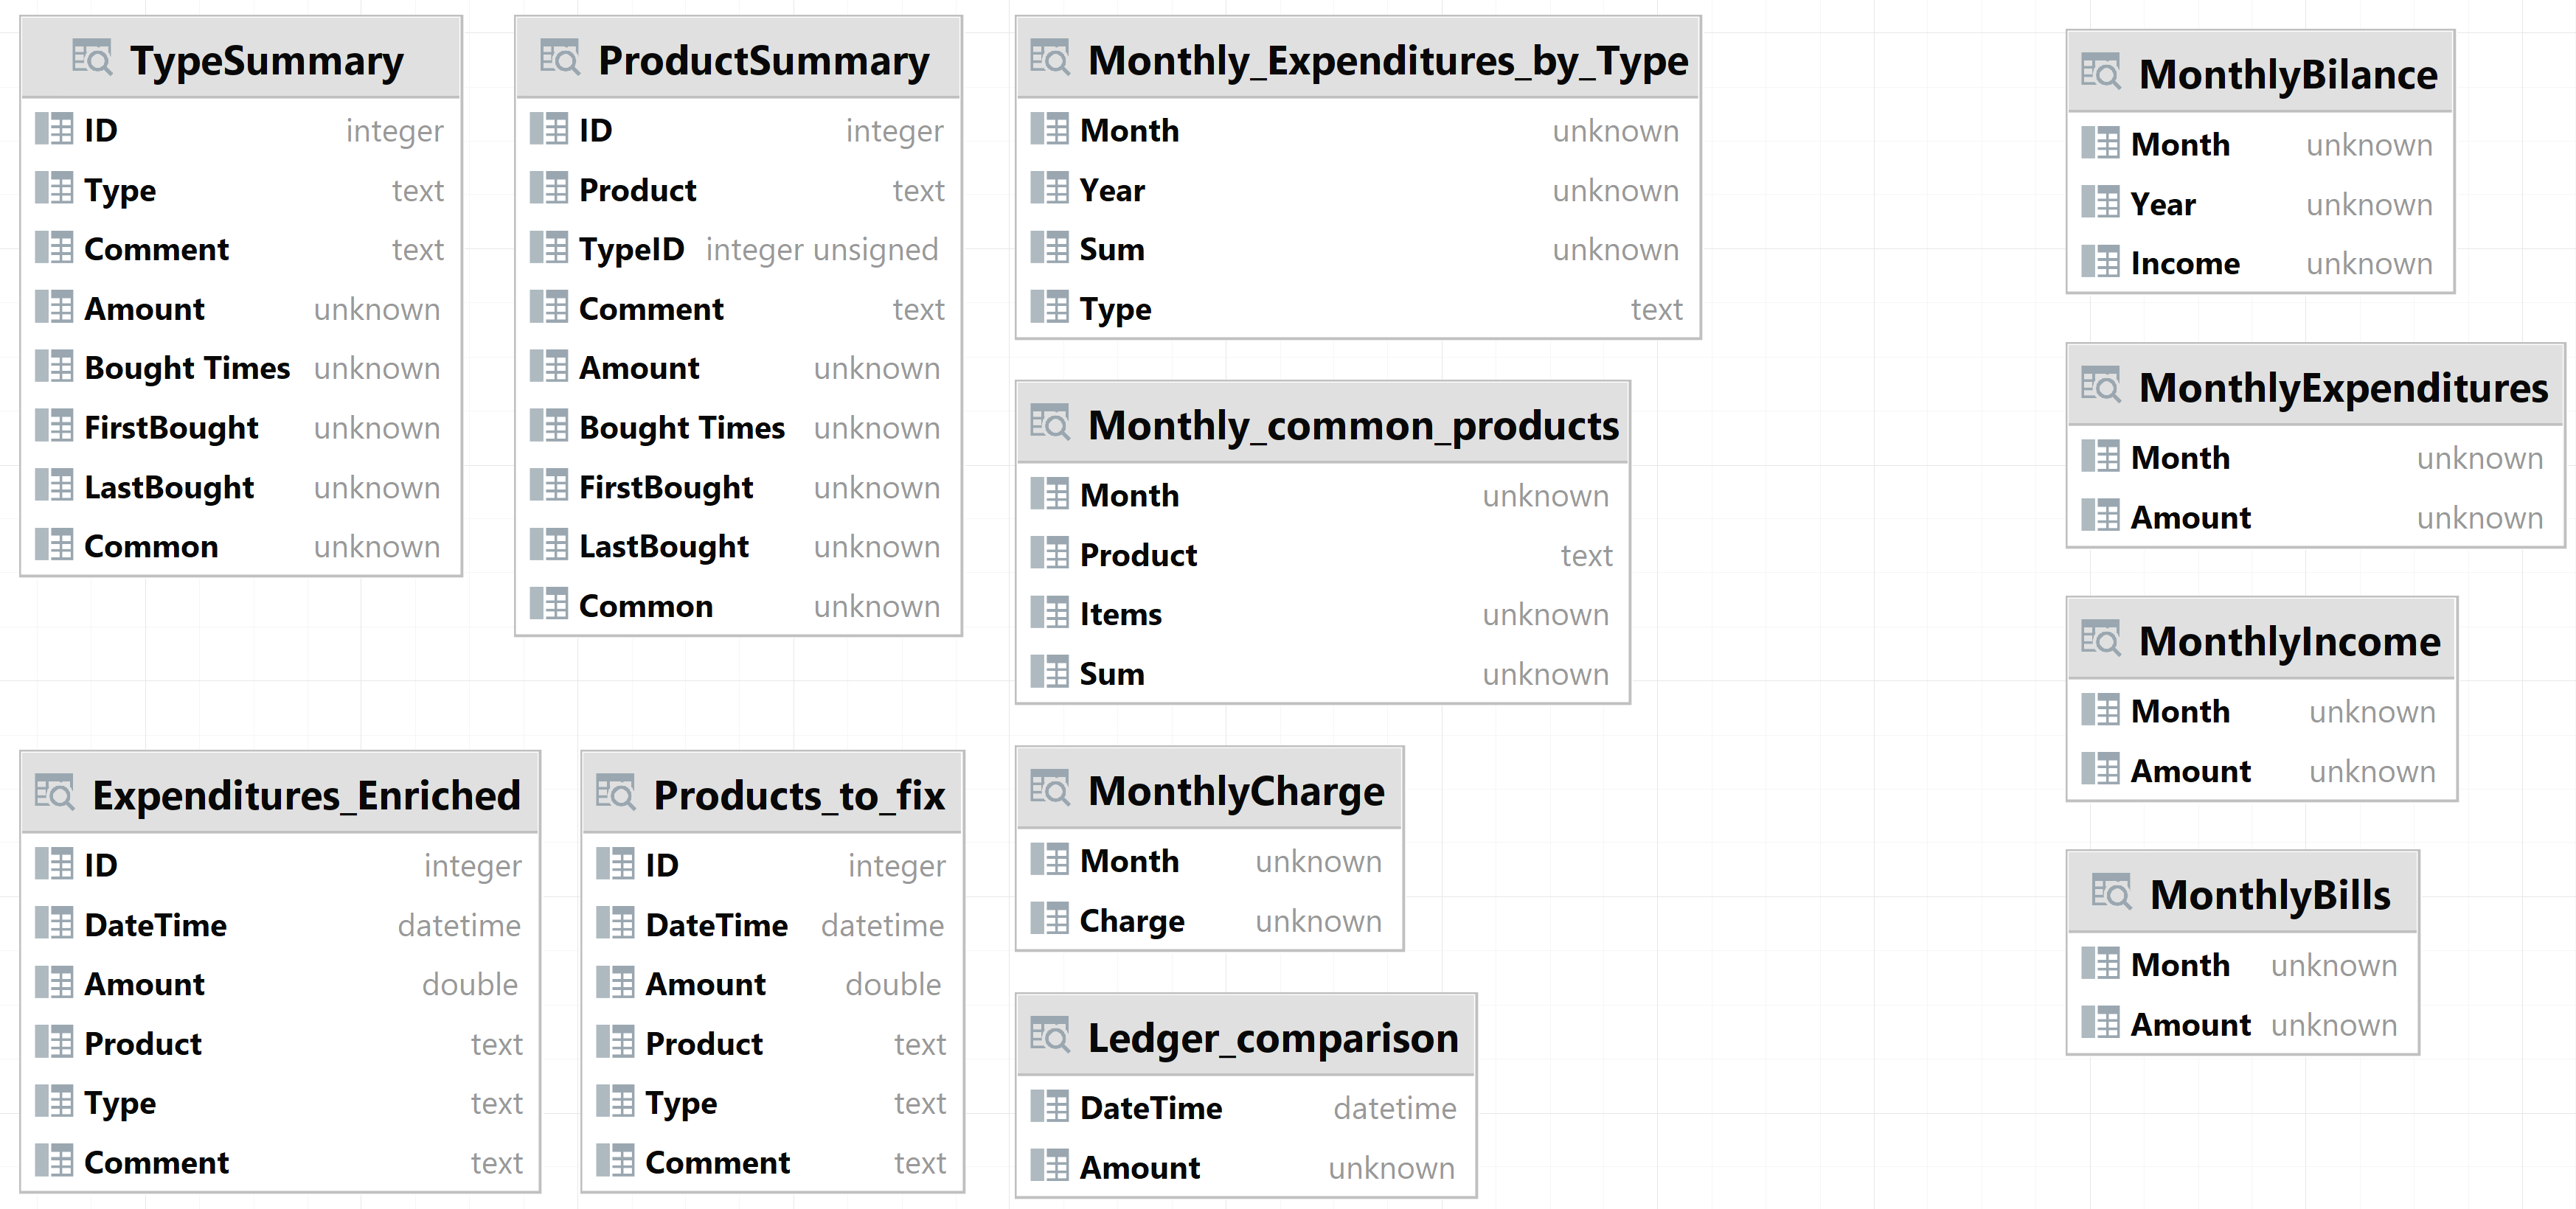
\includegraphics[width=12cm]{figures/Budgeter_Finances-db_Views_DataGrid.png}
\end{figure}

\begin{minipage}{\textwidth}
\begin{lstlisting}[ caption={Widok Expenditures\_Enriched},
    language=SQL,
    deletekeywords={IDENTITY},
    deletekeywords={[2]INT},
    morekeywords={clustered},
    framesep=8pt,
    xleftmargin=40pt,
    framexleftmargin=40pt,
    frame=tb,
    framerule=0pt ]
CREATE VIEW [Expenditures_Enriched] AS
SELECT  [EXP].[ID]          as ID,
        [EXP].[DateTime]    as DateTime,
        [EXP].[Amount]      as Amount,
        [PRD].[Product]     as Product,
        [PTY].[Type]        as Type,
        [EXP].[Comment]     as Comment
FROM  [Expenditures]            [EXP]
LEFT JOIN [Products]            [PRD]	
    ON [EXP].[ProductID]=[PRD].[ID]
LEFT JOIN [ProductTypes]        [PTY]
    ON [PRD].[TypeID]=[PTY].[ID]
ORDER BY DateTime;
\end{lstlisting}
{Widok Expenditures\_Enriched prezentuje użytkownikowi czytelne dane z tabeli 
Expenditures wzbogacone o produkty zdefiniowane w tabeli Products i typy z 
tabeli ProductTypes.}
\end{minipage}

\begin{minipage}{\textwidth}
\begin{lstlisting}[ caption={Widok MonthlyExpenditures},
    language=SQL,
    deletekeywords={IDENTITY},
    deletekeywords={[2]INT},
    morekeywords={clustered},
    framesep=8pt,
    xleftmargin=40pt,
    framexleftmargin=40pt,
    frame=tb,
    framerule=0pt ]
CREATE VIEW [MonthlyExpenditures] AS
SELECT 
    SUBSTR([DateTime], 1, 7)    as [Month]
    ,SUM([Amount])              as [Amount]
FROM [Expenditures_Enriched]
GROUP BY [Month]
ORDER BY [Month];
\end{lstlisting}
{Widok MonthlyExpenditures podsumowuje dane o miesięcznych wydatkach użytkownika.}
\end{minipage}

\begin{minipage}{\textwidth}
\begin{lstlisting}[ caption={Widok MonthlyBills},
    language=SQL,
    deletekeywords={IDENTITY},
    deletekeywords={[2]INT},
    morekeywords={clustered},
    framesep=8pt,
    xleftmargin=40pt,
    framexleftmargin=40pt,
    frame=tb,
    framerule=0pt ]
CREATE VIEW [MonthlyBills] AS
SELECT 
    SUBSTR([DateTime], 1, 7)    as [Month]
    ,SUM([Amount])              as [Amount]
FROM [Bills]
GROUP BY [Month]
ORDER BY [Month];
\end{lstlisting}
{Widok MonthlyBills dane o rachunkach bieżących użytkownika w rozrachunku 
miesięcznym na podstawie danych zawartych w tabeli Bills.}
\end{minipage}

\begin{minipage}{\textwidth}
\begin{lstlisting}[ caption={Widok MonthlyIncome},
    language=SQL,
    deletekeywords={IDENTITY},
    deletekeywords={[2]INT},
    morekeywords={clustered},
    framesep=8pt,
    xleftmargin=40pt,
    framexleftmargin=40pt,
    frame=tb,
    framerule=0pt ]
CREATE VIEW [MonthlyIncome] AS
SELECT
	SUBSTR([DateTime], 1, 7)				as Month
	,SUM([Amount])							as Amount
FROM 	[Income]
GROUP BY [Month]
ORDER BY [Month];
\end{lstlisting}
{Widok MonthlyIncome podsumowuje dane o przychodach użytkownika w ujęciu 
miesięcznym.}
\end{minipage}

\begin{minipage}{\textwidth}
\begin{lstlisting}[ caption={Widok MonthlyBilance},
    language=SQL,
    deletekeywords={IDENTITY},
    deletekeywords={[2]INT},
    morekeywords={clustered},
    framesep=8pt,
    xleftmargin=40pt,
    framexleftmargin=40pt,
    frame=tb,
    framerule=0pt ]
CREATE VIEW [MonthlyBilance] AS 
SELECT 
    Strftime('%Y-%m', [DateTime])   as [Month],
    Strftime('%Y',    [DateTime])   as [Year],
    ROUND(SUM([Amount]), 2)         as [Income]
    --Previous_month_income - (bills + expenditures)
FROM (SELECT 
        DATE(Strftime('%Y-%m-01', [DateTime]),[-1 month]) as [DateTime],
        [Amount]  
      FROM [Income]
      UNION SELECT
                [DateTime], 
                -([Amount]) 
            FROM [Expenditures_Enriched]
      UNION SELECT
                [DateTime],
                -([Amount])
            FROM [Bills])
 GROUP BY [Month]
 ORDER BY [Month] DESC;
\end{lstlisting}
{Widok MonthlyBilance podsumowuje bilans miesięczny wydatków i wpływów 
użytkownika w formie pojedynczej liczby.}
\end{minipage}

\begin{minipage}{\textwidth}
\begin{lstlisting}[ caption={Widok Monthly\_common\_products},
    language=SQL,
    deletekeywords={IDENTITY},
    deletekeywords={[2]INT},
    morekeywords={clustered},
    framesep=8pt,
    xleftmargin=40pt,
    framexleftmargin=40pt,
    frame=tb,
    framerule=0pt ]
CREATE VIEW [Monthly_common_products] AS
SELECT * 
FROM (
    SELECT  Strftime('%Y-%m', [DateTime])   AS [Month],
                                               [Product],
            COUNT([Product])                AS [Items], 
            SUM([Amount])                   AS [Sum]
    FROM [Expenditures_Enriched]
    GROUP BY [Product], [Month]
    ORDER BY [Month] DESC, [Sum] DESC
) WHERE [Items]>=4;
\end{lstlisting}
{Widok Monthly\_common\_products podsumowuje dane o produkach które użykownik 
kupował najczęściej każdego miesiąca. Uwzględnia wyłącznie produkty które 
zakupiono 4 razy - liczbę wybrano arbitralnie metodą kolejnych przybliżeń aby 
otrzymać zadowalający wynik.}
\end{minipage}

\begin{minipage}{\textwidth}
\begin{lstlisting}[ caption={Widok Monthly\_Expenditures\_by\_Type},
    language=SQL,
    deletekeywords={IDENTITY},
    deletekeywords={[2]INT},
    morekeywords={clustered},
    framesep=8pt,
    xleftmargin=40pt,
    framexleftmargin=40pt,
    frame=tb,
    framerule=0pt ]
CREATE VIEW [Monthly_Expenditures_by_Type] AS 
SELECT	Strftime('%Y-%m', [DateTime]) as [Month],
        Strftime('%Y',    [DateTime]) as [Year],
        ROUND(SUM([Amount]), 2)       as [Sum],
        [Type]
FROM (SELECT 
        [DateTime], 
        [Type], 
        [Amount] 
      FROM [Expenditures_Enriched])
GROUP BY [Type], [Month]
ORDER BY [Month] DESC, [Sum] DESC;
\end{lstlisting}
{Widok Monthly\_Expenditures\_by\_Type podsumowuj dane o typach produktów 
zakupionych przez użytkownika w ujęciu miesięcznym.}
\end{minipage}

\begin{minipage}{\textwidth}
\begin{lstlisting}[ caption={Widok Temp\_check},
    language=SQL,
    deletekeywords={IDENTITY},
    deletekeywords={[2]INT},
    morekeywords={clustered},
    framesep=8pt,
    xleftmargin=40pt,
    framexleftmargin=40pt,
    frame=tb,
    framerule=0pt ]
CREATE VIEW [Temp_check] 
    (Temp_ID, Temp_Product, Product_ID)
AS
SELECT *
FROM (SELECT 
        Expenditures_transitory.ID      as [Temp_ID],
        Expenditures_transitory.Product as [Temp_Product],
        Products.ID                     as [Product_ID]
      FROM [Expenditures_transitory]
      LEFT OUTER JOIN [Products]
      ON [Expenditures_transitory].[Product]==[Products].[Product]
)
WHERE [Product_ID] IS NULL;
\end{lstlisting}
{Widok Temp\_check weryfikuje poprawność danych wprowadzonych przez użytkownika.}
\end{minipage}

\begin{minipage}{\textwidth}
\begin{lstlisting}[ caption={Widok Products\_to\_fix},
    language=SQL,
    deletekeywords={IDENTITY},
    deletekeywords={[2]INT},
    morekeywords={clustered},
    framesep=8pt,
    xleftmargin=40pt,
    framexleftmargin=40pt,
    frame=tb,
    framerule=0pt ]
CREATE VIEW [Products_to_fix] AS
SELECT *
FROM [Expenditures_Enriched]
WHERE [Product] IN (NULL,
                    'UNKNOWN')
    OR [Comment] LIKE '%[TODO]%';
\end{lstlisting}
{Widok Products\_to\_fix zawiera dane wprowadzone przez użytkownika poprawnie i 
oznaczone jako dane do uzupełnienia specjalnymi etykietami - wartością w polu 
PRODUCT=UNKNOWN lub [TODO] w komentarzu.}
\end{minipage}

\begin{minipage}{\textwidth}
    \begin{lstlisting}[ caption={Widok TypeSummary},
        language=SQL,
        deletekeywords={IDENTITY},
        deletekeywords={[2]INT},
        morekeywords={clustered},
        framesep=8pt,
        xleftmargin=40pt,
        framexleftmargin=40pt,
        frame=tb,
        framerule=0pt ]
    CREATE VIEW IF NOT EXISTS [TypeSummary] AS
    SELECT
        [ProductTypes].[ID]                         AS [ID]
        ,[ProductTypes].[Type]                    AS [Type]
        ,[ProductTypes].[Comment]              AS [Comment]
        ,IFNULL([Summary].[Amount], 0)          AS [Amount]
     ,IFNULL([Summary].[Bought Times], 0) AS [Bought Times]
        ,[Summary].[FirstBought]           AS [FirstBought]
        ,[Summary].[LastBought]             AS [LastBought]
        ,IFNULL([Summary].[Common], 'Absent')   AS [Common]
    FROM [ProductTypes]
    LEFT JOIN (SELECT 
        *
        ,(CASE WHEN ([Bought Times]>(
            SELECT 
                AVG([Bought Times]) AS [Average] 
            FROM (SELECT
                    [Type]
                    ,Round(SUM([Amount]), 2) AS [Amount]
                    ,COUNT([DateTime]) AS [Bought Times]
                    ,MAX([DateTime])     AS [LastBought]
                    ,MIN([DateTime])    AS [FirstBought]
                FROM [Expenditures_Enriched]
                GROUP BY [Type]
                ORDER BY [Bought Times] DESC))) 
        then 'Common' else 'Uncommon' end) as [Common]
        
    FROM (	SELECT
               [Type]
               ,Round(SUM([Amount]), 2) AS [Amount]
               ,COUNT([DateTime])       AS [Bought Times]
               ,MAX(DateTime)           AS [LastBought]
               ,MIN(DateTime)           AS [FirstBought]
            FROM [Expenditures_Enriched]
            GROUP BY [Type]
            ORDER BY [Bought Times] DESC))
    AS [Summary]
    ON [ProductTypes].[Type]=[Summary].[Type];
    \end{lstlisting}
    {Widok TypeSummary podsumowuj dane o typach produktów użytkownika.}
    \end{minipage}
    
    \begin{minipage}{\textwidth}
        \begin{lstlisting}[ caption={Widok ProductSummary},
            language=SQL,
            deletekeywords={IDENTITY},
            deletekeywords={[2]INT},
            morekeywords={clustered},
            framesep=8pt,
            xleftmargin=40pt,
            framexleftmargin=40pt,
            frame=tb,
            framerule=0pt ]
    CREATE VIEW IF NOT EXISTS [ProductSummary] AS
    SELECT
        [Products].[ID]                             AS [ID]
        ,[Products].[Product]                  AS [Product]
        ,[Products].[TypeID]                    AS [TypeID]
        ,[Products].[Comment]                  AS [Comment]
        ,IFNULL([Summary].[Amount], 0)          AS [Amount]
     ,IFNULL([Summary].[Bought Times], 0) AS [Bought Times]
        ,[Summary].[FirstBought]           AS [FirstBought]
        ,[Summary].[LastBought]             AS [LastBought]
        ,IFNULL([Summary].[Common], 'Absent')   AS [Common]
    FROM [Products]
    LEFT JOIN (SELECT 
        *
        ,(CASE WHEN ([Bought Times]>(
            SELECT 
                AVG([Bought Times]) AS [Average] 
            FROM (SELECT
                    [Product]
                    ,Round(SUM([Amount]), 2) AS [Amount]
                    ,COUNT([DateTime]) AS [Bought Times]
                    ,MAX([DateTime])     AS [LastBought]
                    ,MIN([DateTime])    AS [FirstBought]
                FROM [Expenditures_Enriched]
                GROUP BY [Product]
                ORDER BY [Bought Times] DESC))) 
        then 'Common' else 'Uncommon' end) as [Common]
        
    FROM (	SELECT
               [Product]
               ,Round(SUM([Amount]), 2) AS [Amount]
               ,COUNT([DateTime])       AS [Bought Times]
               ,MAX(DateTime)           AS [LastBought]
               ,MIN(DateTime)           AS [FirstBought]
            FROM [Expenditures_Enriched]
            GROUP BY [Product]
            ORDER BY [Bought Times] DESC))
    as [Summary]
    ON [Products].[Product]=[Summary].[Product];
    \end{lstlisting}
    {Widok ProductSummary podsumowujący dla użytkownika statystyki produktów.}
    \end{minipage}

%------------------------- Application layer ----------------------------------- 
\section{\customstylesection{Logika aplikacji}} \label{Logika aplikacji}
{W toku prac stopniowo wykorzystywane w projekcie zmienne w formie kolekcji 
słowników  zamieniano w klasy które spajają dane. Wyłoniły się one w wyniku 
refaktoryzacji i tworzenia abstrakcji upraszczających interfejs funkcji. Klasy 
projektowano tak, by były w miarę możliwości oczywiste i zrozumiałe, co ma na 
celu poprawić czytelność i zrozumiałość kodu.}

\begin{minipage}{\textwidth}
    \begin{lstlisting}[ caption={Klasa Database},
        language=Python,
        deletekeywords={IDENTITY},
        deletekeywords={[2]INT},
        morekeywords={clustered},
        framesep=8pt,
        xleftmargin=40pt,
        framexleftmargin=40pt,
        frame=tb,
        framerule=0pt ]
class Database():
    def __init__(self, 
                 fullpath,
                 schema,
                 selects, 
                 inserts,
                 updates):
        self.fullpath = fullpath
        self.schema = schema
        self.selects = selects
        self.inserts = inserts
        self.updates = updates
    \end{lstlisting}
{Obiekty klasy Database zawierają komplet informacji wymaganych do interakcji z
 bazą danych wykorzystwaną w aplikacji. Pole fullpath to w pełni kwalifikowana
 ścieżka do bazy danych, schema jest kolekcją obiektów typu string która 
przechowuje schemat bazy danych. Pozostałe pola: selects, inserts, updates to 
słowniki które pozwalają po nazwie odwołać się do odpowiednio zapytań (SELECT), 
dodawania rekordów do tabel (INSERT), oraz aktualizacji danych w tabelach 
(updates).}
\end{minipage}

\begin{minipage}{\textwidth}
    \begin{lstlisting}[ caption={Klasa ChartSelect},
        language=Python,
        deletekeywords={IDENTITY},
        deletekeywords={[2]INT},
        morekeywords={clustered},
        framesep=8pt,
        xleftmargin=40pt,
        framexleftmargin=40pt,
        frame=tb,
        framerule=0pt ]
class ChartSelect():
    def __init__(self,
                 database,
                 select,
                 label
                ):
        self.database=str(database),
        self.select=str(select),
        self.label=str(label)
    \end{lstlisting}
{Obiekty klasy ChartSelect posiadają trzy atrybuty typu string: database
 przechowuje w pełni kwalifikowaną ścieżkę do bazy danych aplikacji, select 
to zapytanie SQL do bazy, natomiast pole label to etykieta wykresu danych 
wyświetlanego użytkownikowi.}
\end{minipage}

\begin{minipage}{\textwidth}
    \begin{lstlisting}[ caption={Klasa Chart},
        language=Python,
        deletekeywords={IDENTITY},
        deletekeywords={[2]INT},
        morekeywords={clustered},
        framesep=8pt,
        xleftmargin=40pt,
        framexleftmargin=40pt,
        frame=tb,
        framerule=0pt ]
class Chart():
    def __init__(self,
                 selects,
                 caption):
        self.selects = selects
        self.caption = caption
    \end{lstlisting}
{Obiekty klasy Chart definiują dane do wizualizacji. Atrybut caption przyjmuje 
wartości typu string wyświetlane jako nagłówek wizualizacji, natomiast atrybut 
selects jest listą obiektów typu ChartSelect - zbioru zapytań które zostaną 
wyświetlone w ramach pojedynczej wizualizacji.}
\end{minipage}

\label{Classes-CellEdition}
\begin{minipage}{\textwidth}
    \begin{lstlisting}[ caption={Klasa CellEdition},
        language=Python,
        deletekeywords={IDENTITY},
        deletekeywords={[2]INT},
        morekeywords={clustered},
        framesep=8pt,
        xleftmargin=40pt,
        framexleftmargin=40pt,
        frame=tb,
        framerule=0pt ]
class CellEdition():
    def __init__(self,
                 table, 
                 ID, 
                 field, 
                 newvalue,
                 oldvalue): 
        self.table = table
        self.ID = ID
        self.field = field
        self.newvalue = newvalue
        self.oldvalue = oldvalue

    def __repr__(self): 
        return "Table % s modified. ID: % s field: % s oldvalue: % s newvalue: % s" % (self.table, 
                 self.ID, 
                 self.field, 
                 self.newvalue,
                 self.oldvalue)
    \end{lstlisting}
{Obiekty klasy CellEdition przechowują dane edytowanego przez użytkownika 
używającego interfejsu aplikacji rekordu bazy danych. Każdy obiekt przechowuje w
 polach odpowiednio:}
\begin{itemize}
    \item table - tabelę któej dotyczy zmiana
    \item ID - identyfikator modyfikowanego rekordu
    \item field - pole które jest zmieniane
    \item newvalue - nowa wartość pola
    \item oldvalue - wartość pola przed zmianą
\end{itemize}
{Funkcja składowa \inlinecode{\_\_repr\_\_} formatuje dane które zawiera obiekt 
do ciągu znaków. Obecnie używana wyłacznie do logowania wpisu na standardowe 
wyjście, aplikacji. Możliwe że w późniejszych etapach zostanie wykorzystana do 
rejestrowania zdarzenia w logu aplikacji.}
\end{minipage}

\section{\customstylesection{Graficzny interfejs użytkownika}} 
\label{Graficzny interfejs użytkownika}
{Graficzny interfejs użytkownika (GUI, Graphical User interface) aplikacji 
utworzono z wykorzystaniem biblioteki PySimpleGUI \cite{PySimpleGUI}. Dzięki 
temu interfejs definiowany jest w postaci kolekcji jak listy, lub listy list, 
obiektów klas zawartych w bibliotece - jako przykład przedstawiono opcje listy 
rozwijanej na poniższym listingu. %TODO: Figure out how to reference listings \ref{Dropdown}. 
Aby zapewnić responsywność interfejs budowany jest w kilku etapach, a cała 
budowa wydzielona do specjalnych funkcji generujących wywoływanych później 
zależnie od potrzeb. Funkcje opisane są w dalszej części w sekcji 
\nameref{Metody projektu}.}

\begin{minipage}{\textwidth}
    \begin{lstlisting}[ caption={Lista rozwijana przykład definicji interfejsu},
        language=Python,
        deletekeywords={IDENTITY},
        deletekeywords={[2]INT},
        morekeywords={clustered},
        framesep=8pt,
        xleftmargin=40pt,
        framexleftmargin=40pt,
        frame=tb,
        framerule=0pt ]
    menu = [['Visualizations', 
                ['Most common products', 
                 'Income summary',
                 'Monthly Bilance',
                 'TopTypeMonthly',
                 'Type'
                    ,[types],
                 'Product'
                    ,[products]]],
            ['Browse data',
                #TODO: Add views as uneditable
                ['Expenditures',
                 'Bills',
                 'Income',
                 'Types' ,
                 'Products',]],
            ['Options',
                [#'Configure',
                 'Change Theme',
                    [themes],
                'Version',
                'About...',
                'Manual']] #TODO: Wishful thinking - built in manual
            ]
    \end{lstlisting}
\end{minipage}

{Interfejs przedstawiono poglądowo na poniższyczh grafikach.}
%{Jego iteracyjny rozwój zaprezentowano na przykładzie zakładki Visualizations.} %TODO: optional
\begin{figure}[H]           %requires float package
    \caption{Wizualizacja danych}
    \label{fig:Wizualizacja danych}
    \centering  
    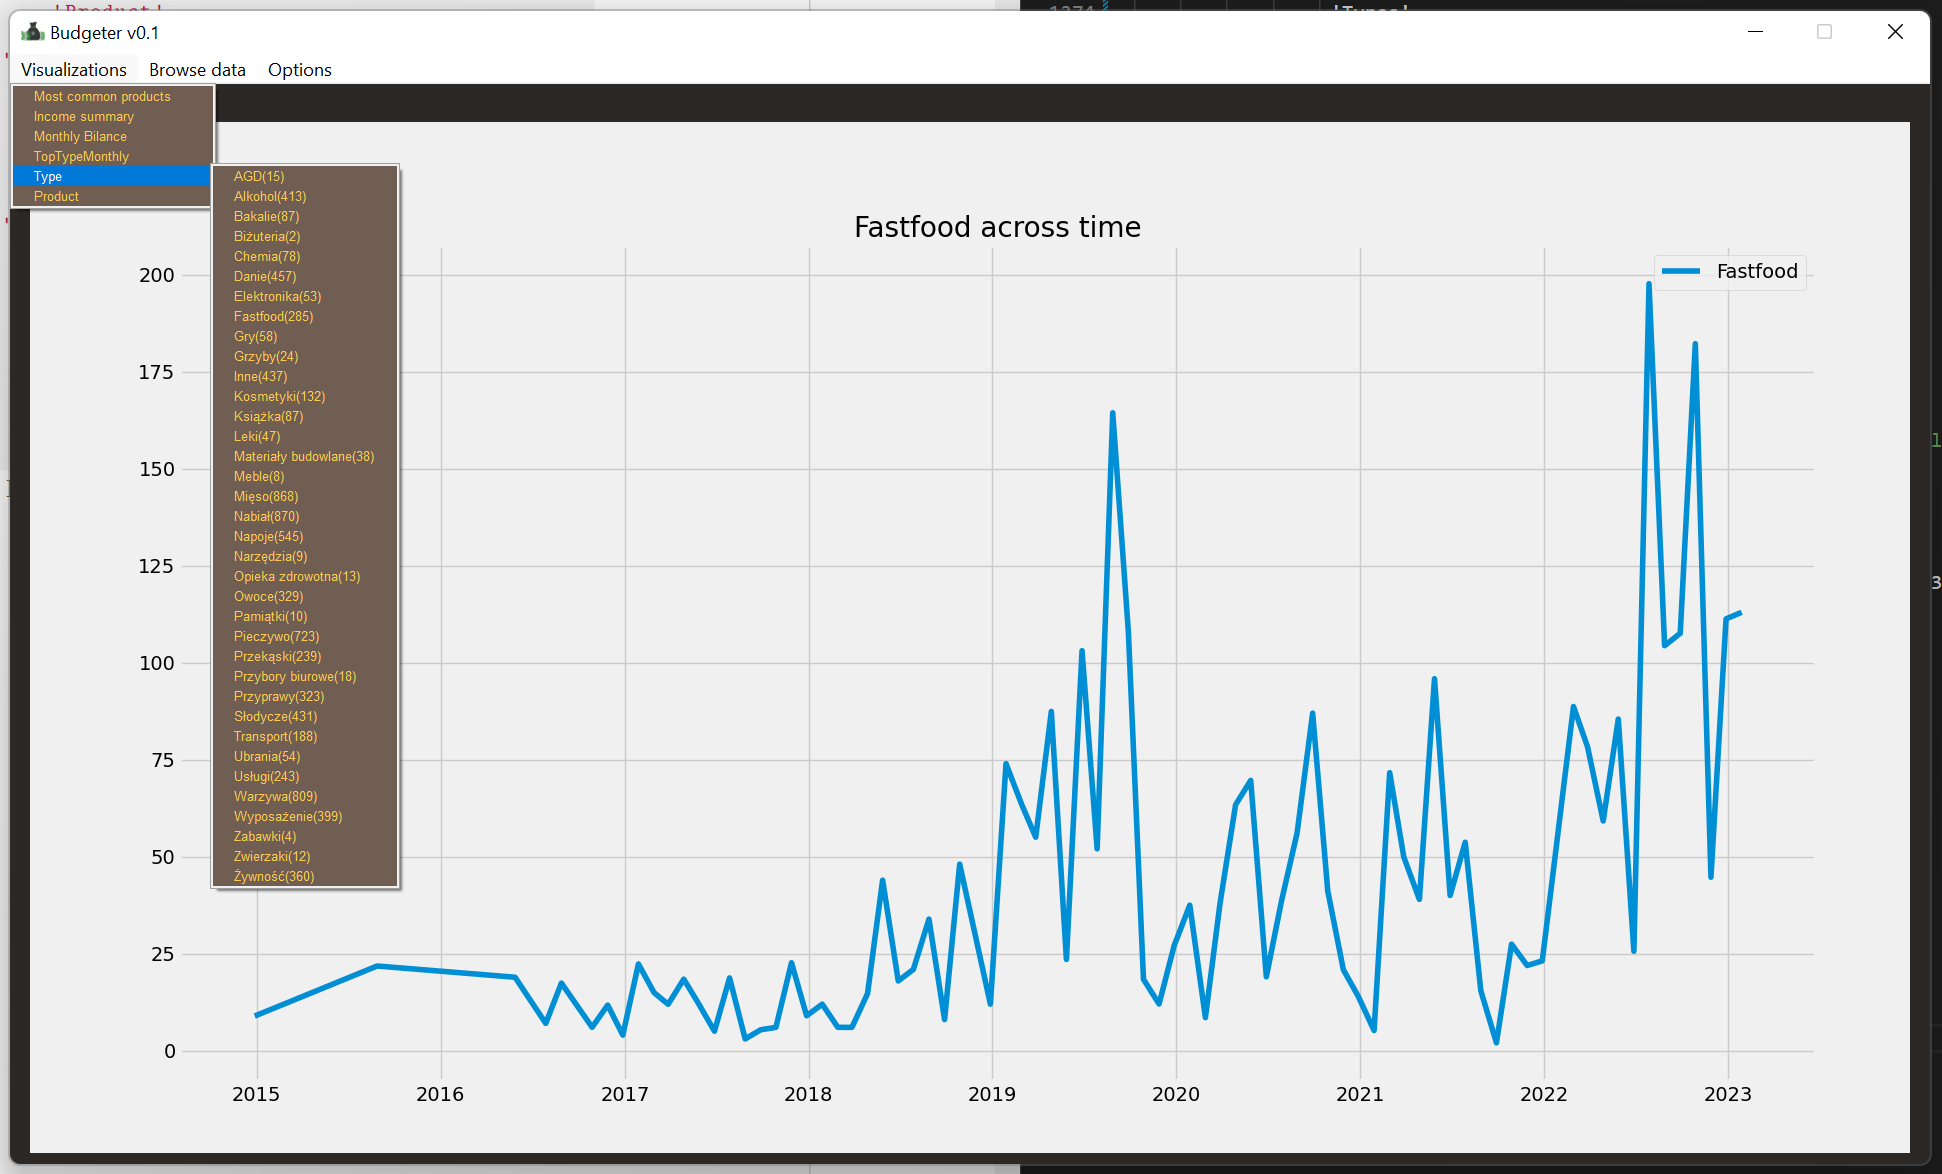
\includegraphics[width=12cm]{figures/Interface_Visualizations_v0.3.png}
\end{figure}

\begin{figure}[H]           %requires float package
    \caption{Opcje}
    \label{fig:Opcje}
    \centering  
    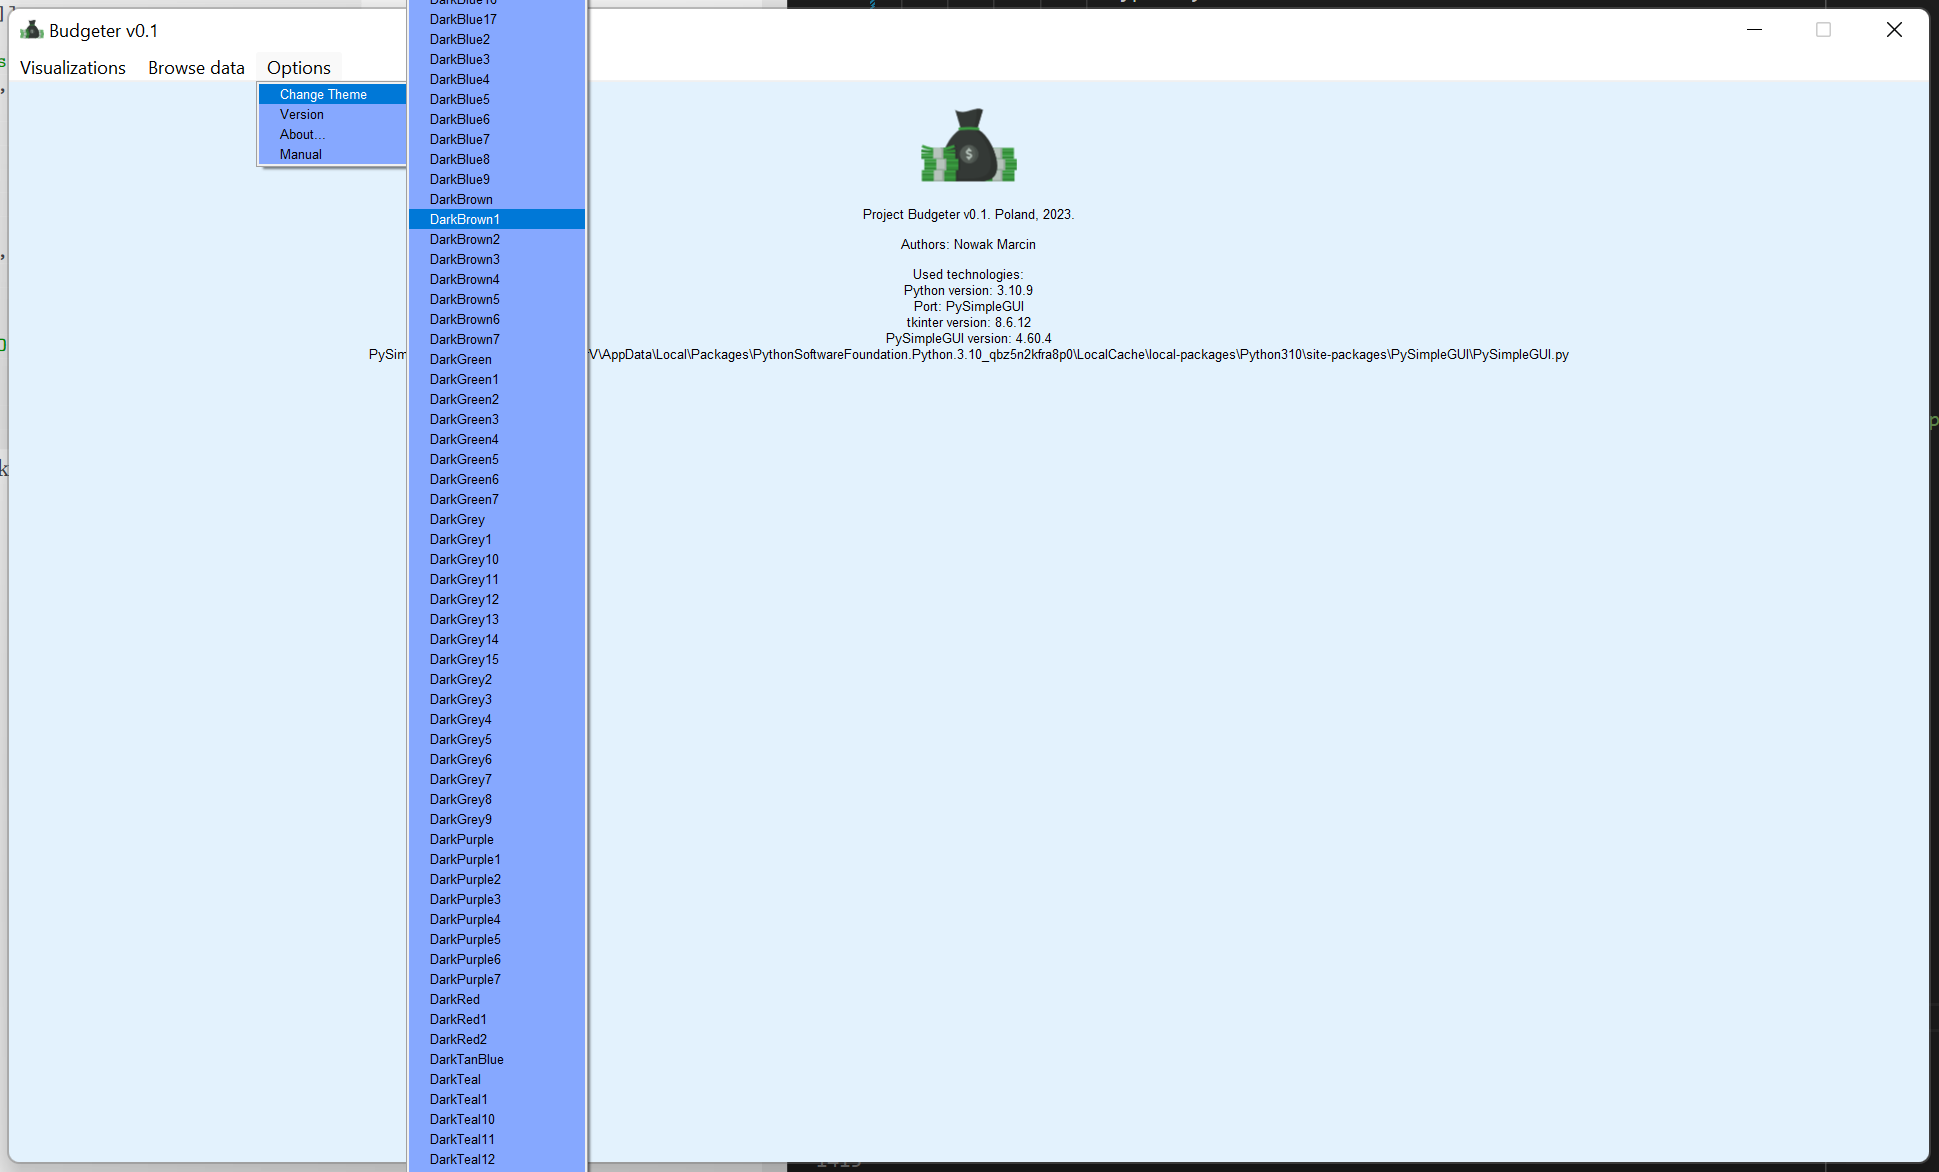
\includegraphics[width=12cm]{figures/Interface_Options_v0.3.png}
\end{figure}

\begin{figure}[H]           %requires float package
    \caption{Import danych}
    \label{fig:Import danych}
    \centering  
    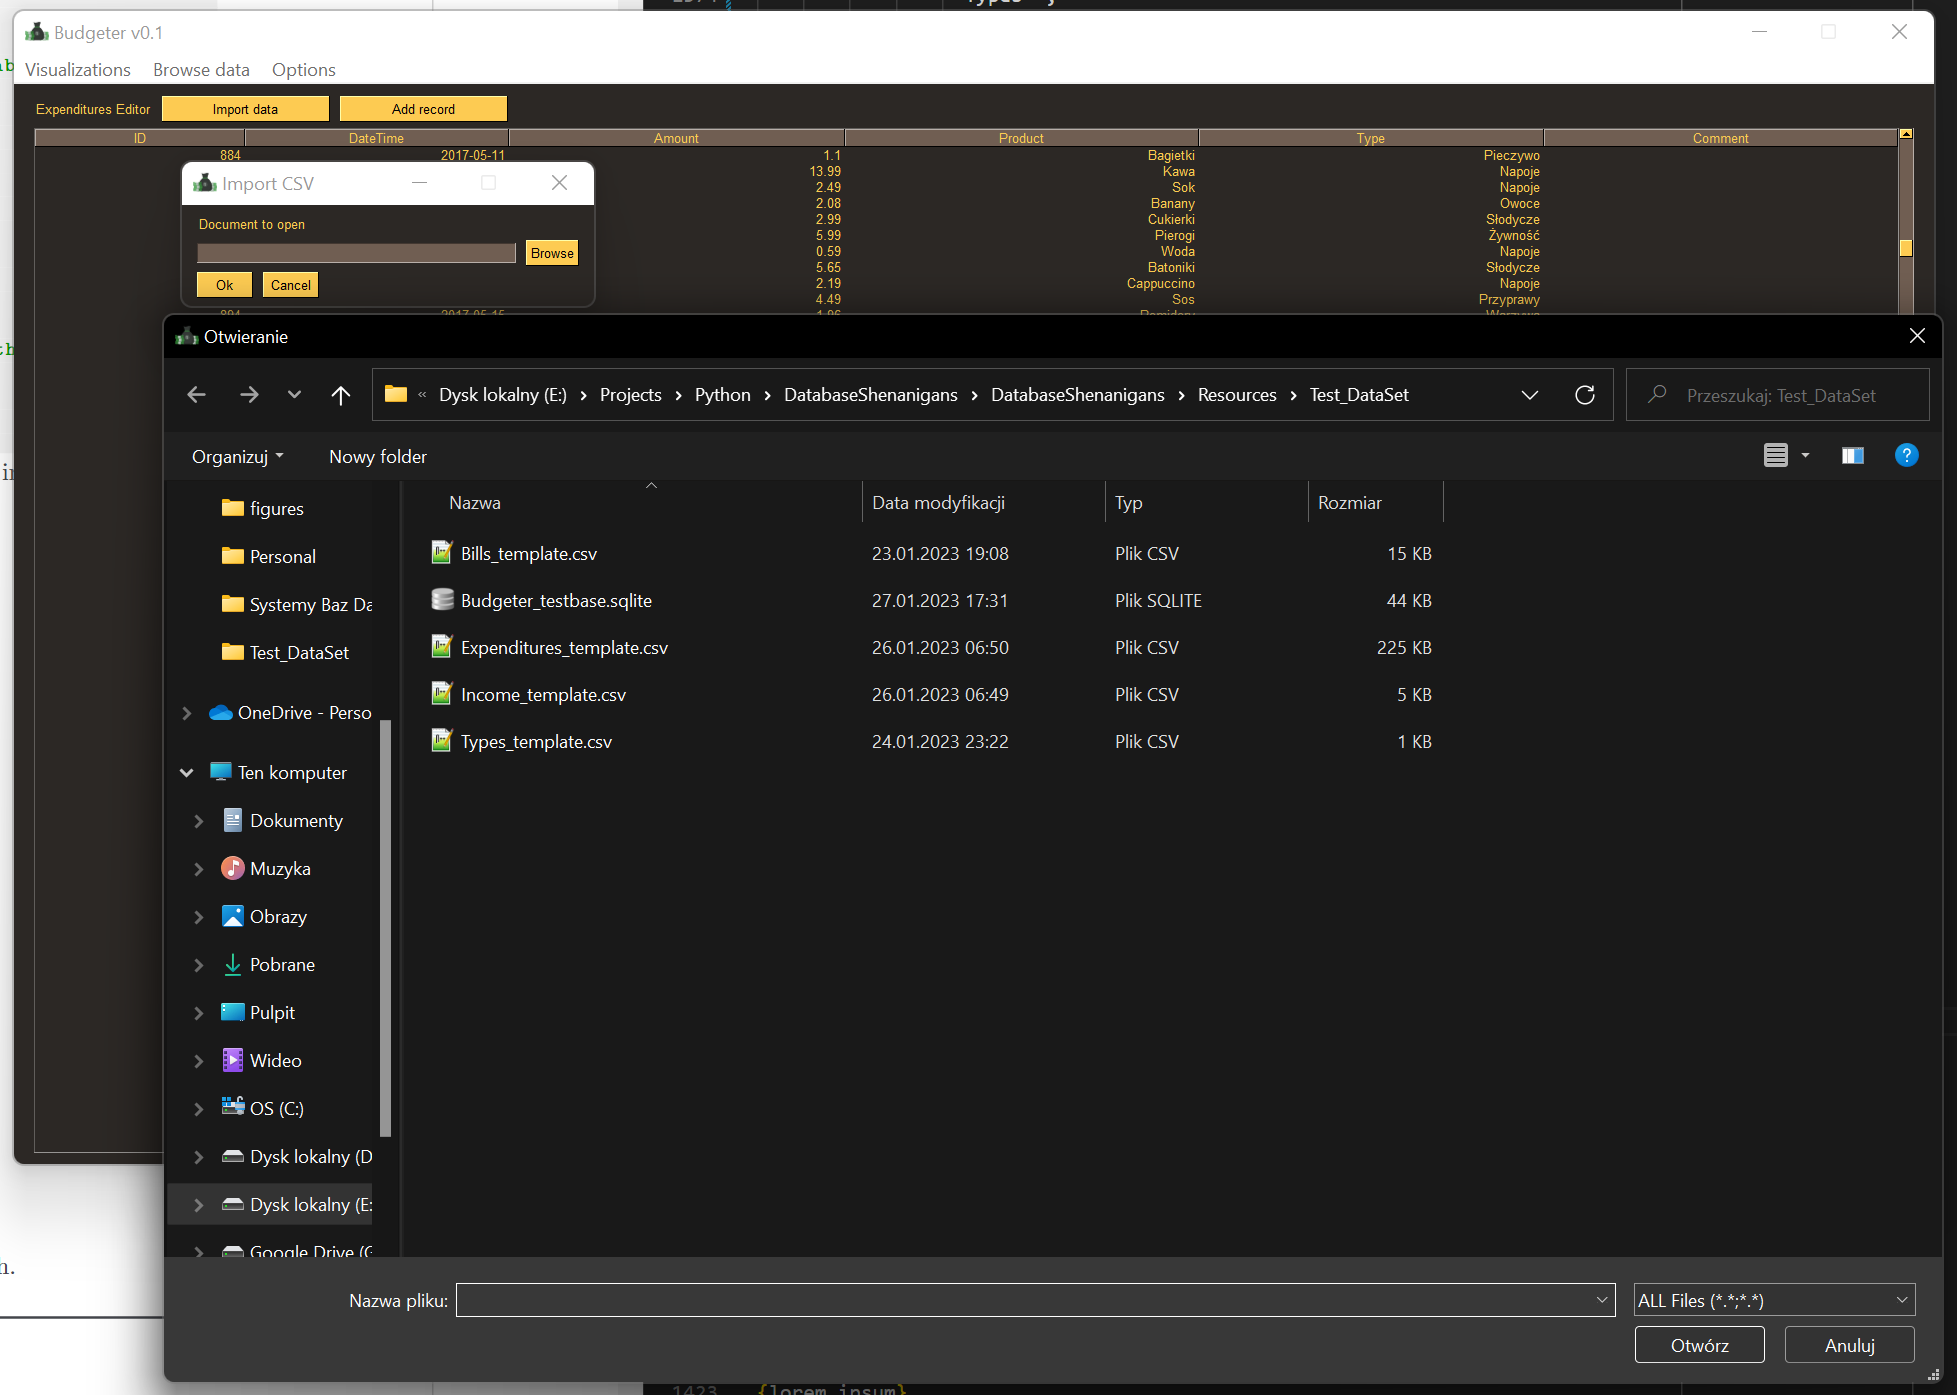
\includegraphics[width=12cm]{figures/Interface_Browse_Import_v0.3.png}
\end{figure}

\begin{figure}[H]           %requires float package
    \caption{Dodawanie rekordu}
    \label{fig:Dodawanie rekordu}
    \centering  
    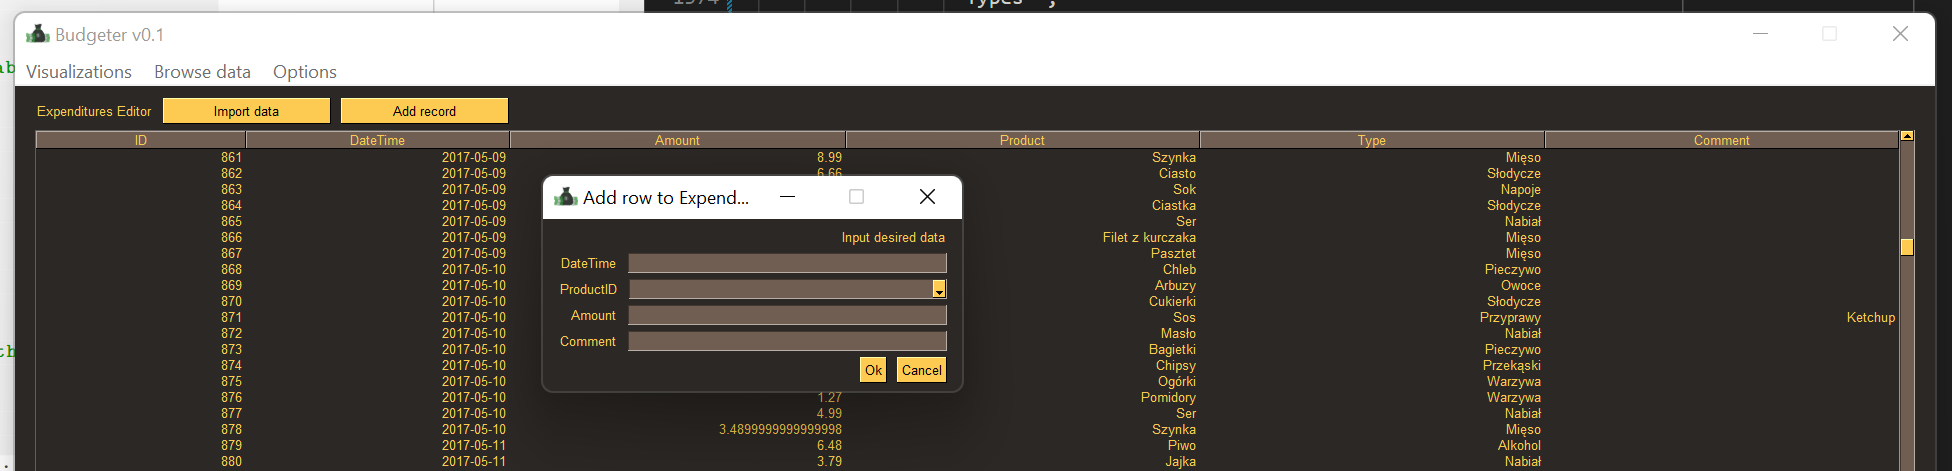
\includegraphics[width=12cm]{figures/Interface_Browse_AddRecord_v0.3.png}
\end{figure}

\section{\customstylesection{Metody projektu}} 
\label{Metody projektu}
{Kod aplikacji podzielono na funkcje aby zgodnie z dobrymi praktykami zebrać 
logikę realizującą konkretne zadanie w jednym miejscu.}

\medskip
{Funkcja \inlinecode{PrepareStatement(query, values)} przygotowuje i zwraca 
zapytania dodające lub modyfikujące jeden lub wiele rekordów bazy danych na 
podstawie zapytania podanego w argumencie \inlinecode{query} i tablicy wartości 
w argumencie \inlinecode{values}.}

\medskip
{Funkcja \inlinecode{GetFromDB(database, select)} pobiera dane z bazy wskazanej 
argumentem \inlinecode{database} zapytaniem podanym jako argument 
\inlinecode{select}. Oba argumenty są typu string. Zwraca dane jako tablicę 
złożoną z poszczególnych pól tablicy w bazie jako pola i poszczególnych 
wpisów w jako rekordów.}

\medskip
{Procedura \inlinecode{SendToDB(database, todb)} wysyła dane do bazy wskazanej
argumentem \inlinecode{database} zapytaniem podanym jako argument 
\inlinecode{select}. Oba argumenty są typu string. Nie zwraca wartości.}

\medskip
{Funkcja \inlinecode{GetCollectionFromDB(collection)} przyjmuje jako argument 
\inlinecode{collection} obiekt klasy Chart który zawiera listę złożoną z zapytań
 do bazy i odpowiadających im opisów wykresów. Funkcja ta zwraca listę krotek 
złożonych z tablicy danych pobranych z bazy funkcją \inlinecode{GetFromDB} oraz 
ciągu znaków klasy string z etykietą danych prezentowaną na wykresie.}

\medskip
{Funkcja \inlinecode{GetDBInfo(database)} w argumencie \inlinecode{database} 
przyjmuje ciąg znaków który jest ścieżką do bazy danych. Wykorzystując funkcję 
\inlinecode{GetFromDB} oraz predefiniowane zapytania buduje pobiera schemat bazy
 pobierając listę dostępnych tabel i widoków, a następnie nazwy kolumn każdej z 
nich. Tak zebrane dane tworzą słownik w którym pod nazwą danej tabeli lub 
indeksem w słowniku kryje się obiekt z nazwą tablicy jako parametr name, i listą
 kolumn w polu columns.}

\medskip
{Funkcja \inlinecode{Prepare\_plot(set, title)} przetwarza dane do wykresu. 
Przyjmuje w argumencie \inlinecode{set} listę tablic złożonych z listy dat w 
formie ciagu znaków klasy strting i wartości liczbowych, i pojedynczego ciągu 
znaków który stanie się etykietą wykresu - dane zwrócone z funkcji 
\inlinecode{GetCollectionFromDB}. Parsuje daty każdego rekordu do odpowiedniego 
formatu przy pomocy zewnętrznej biblioteki. Następnie z danych tworzona jest 
linia wykresu oznaczona etykietą. Na koniec linie łaczone są w jeden wykres, a 
argument \inlinecode{title} przypisywany jest jako jego nagłówek - tak 
przygotowany wykres jest zwracany przez funkcję.}

\medskip
{Funkcja \inlinecode{draw\_figure(canvas, figure)} przetwarza obiekt danych 
wykresu dostarczony w argumencie \inlinecode{figure} na grafikę prezentowaną w 
specjalnym elemencie interfejsu wskazanym w argumencie \inlinecode{canvas}. 
Zwraca referencję do tak przygotowanego obiektu na ekranie.}

\medskip
{Funkcja \inlinecode{Listfromtable(table, addvalues=True)} tworzy z danych 
tablicy podanej w argumencie \inlinecode{table} listę, jeśli wywołano ją z 
argumentem \inlinecode{addvalues}, lub nie podano tego argumentu wogóle, 
dopisuje w nawiasach wartości z tabeli. Zwraca tak utworzoną listę ciągów znaków
 klasy string.}

\medskip
{Funkcja \inlinecode{PrepareCharts()} wstępnie dynamicznie przetwarza część 
zapytań wywoływanych z interfejsu. Tworzy obiekty klasy ChartSelect - pobiera 
dane z bazy o kilku najpopularniejszych produktach, dane o najczęściej kupowanym
 typie produktu, dane o przychodach w ujęciu miesięcznym oraz bilansie 
miesięcznym przychdó i wydatków. Tak przygotowany słownik obiektów złożony z 
nazw w formie ciągów znaków klasy string i przypisanych im obiektów klasy 
ChartSelect jest zwracany.}

\medskip
{Funkcja \inlinecode{GivenProduct(product)} przygotowuje w całości obiekt klasy 
Chart reprezentujący zapytanie do bazy o podsumowanie danych produktu wskazanego
 w argumencie \inlinecode{product}, po czym wyciąga wskazane dane z bazy funckją 
\inlinecode{GetCollectionFromDB}, przygotowuje wykres funkcją 
\inlinecode{Prepare\_plot(set, title)} i zwraca go do wyświetlenia.}

\medskip
{Funkcja \inlinecode{GivenType(type)} przygotowuje w całości obiekt klasy 
Chart reprezentujący zapytanie do bazy o podsumowanie danych typu produktów 
wskazanego w argumencie \inlinecode{type}, po czym wyciąga wskazane dane z bazy 
funckją \inlinecode{GetCollectionFromDB}, przygotowuje wykres funkcją 
\inlinecode{Prepare\_plot(set, title)} i zwraca go do wyświetlenia.}

\medskip
{Funkcja \inlinecode{Visualize(chart)} przyjmuje dane klasy Chart jako argument 
\inlinecode{chart}, wyciąga wskazane dane z bazy funckją 
\inlinecode{GetCollectionFromDB}, przygotowuje wykres funkcją 
\inlinecode{Prepare\_plot(set, title)} i zwraca go do wyświetlenia.}

\medskip
{Funkcja \inlinecode{TableToLayout(table)} tworzy na podstawie tabeli podanej w 
argumencie \inlinecode{table} obiekt biblioteki PySimpleGUI - tablicę osadzaną w
 interfejsie użytkownika.}

\medskip
{Funkcja \inlinecode{GenerateTableEditor(table)} tworzy i zwraca interfejs 
edycji tabeli wskazanej w argumencie \inlinecode{table} w formie ciągu znaków 
klasy string. Na interfejs składają się: tytuł, przycisk Import Data do importu 
danych z pliku, przycisk Add record wywołujący okno dodawania rekodru do tabeli 
oraz osadzoną tabelę uzyskaną wywołaniem funkcji \inlinecode{TableToLayout}.}

\medskip
{Funkcja \inlinecode{TableInputWindow(name)} tworzy okno aplikacji służące do 
edycji danych w tabeli wskazanej atrybutem \inlinecode{name} który jest ciągiem 
znaków klasy string. Funkcja wykorzystuje dane o schemacie bazy do zbudowania 
listy pól do wprowadzania danych przez użytkownika. Jeśli napotka pola 
zawierające identyfikatory które są odwołaniem do innych tabel podmienia je na 
listę rozwijaną która prezentuje użytkownikowi wyłącznie prawidłowe wartości 
jako nazwy, natomiast ich wybranie przypisuje w danym polu odpowiadającą mu 
wartość ID. Funkcja otwiera tak przygotowane okno i zwraca rekord jako słownik 
w którym nazwa kolumny jest indeksem a wartość wpisanym przez użytkownika 
tekstem w polu.}

\medskip
{Funkcja \inlinecode{ChangeLayout(window, element)} zmienia interfejs 
użytkownika. Na okno aplikacji składa się kilka zakładek z których jednocześnie 
tylko jedna z nich jest aktywna. Funkcja wyłącza obecny aktywny element w oknie 
wskazanym argumentem \inlinecode{window}, iaktywuje element wskazany argumentem 
\inlinecode{element} co skutkuje zmianą interfejsu użytkownika wyświetlanego na 
ekranie.}

\medskip
{Funkcja \inlinecode{GetDataFromCSV(filename)} wczytuje dane z pliku CSV którego
 ścieżkę podano w argumencie \inlinecode{filename}. Funkcja dostosowana jest do 
obsługi tabel bazy projektu, dlatego zwracany obiekt jest krotką - pierwsza 
linia pliku traktowana jest jako nagłówek, pozostała zawartość jako dane.}

%TODO: Edit in case if implemented before deadline
\medskip
{Funkcja \inlinecode{EditCell(window, key, row, col, edition)} jest funkcją 
dodatkową wyykraczającą poza ramy podstawowego prototypu aplikacji. Pozwala 
użytkownikowi modyfikować pole rekordu istniejącego w tabeli bazy danych 
apliacji poprzez kliknięcie na wyświtlony w itnerfejsie rekord. Jako parametry 
przyjmuje kolejno: w atrybucie \inlinecode{window} okno z którym użytkownik 
wszedł w interakcję, w atrybucie \inlinecode{key} nazwę tabeli któa jest element
 wywołującym akcję, wartości numeryczne w atrybutach \inlinecode{row} i 
\inlinecode{col} które wskazują edytowaną komórkę, i wreszcie w atrybucie 
\inlinecode{edition} nową wartość wskazanego pola.}

{Finalnie funkcja nie została udostępniona ponieważ bezpośrednio wykorzystuje 
biblioteki niskopoziomowe używane w ramach obiektu który reprezentuje element 
interfejsu biblioteki PySimpleGUI, co wymaga zapoznania się z ich specyfiką i 
zmniejszenia poziomu abstrakcji systemu. Z uwagi na edukacyjny charakter 
projektu oraz ograniczone ramy czasowe implementacji planowanych rozwiązań, 
uznano że funckja ta jest zbyt wymagająca.}

\medskip
{Funkcja \inlinecode{PrepareWindow(theme=chosentheme)} przygotowuje główne okno 
aplikacji. Jako jedyny argument \inlinecode{theme} przyjmuje ciąg znaków klasy 
string który jest nazwą jednego z dostępnych w bibliotece motywów, a jego 
wartość domyślna jest zapisana w pliku konfiguracyjnym. Gotowe wygenerowane okno
 jest zwracane do głównej pętli programu która odczytuje działania użytkownika i
 podejmuje odpowiednie akcje.}

\section{\customstylesection{Obiekty projektu}}
{Projekt w trakcie działania wykorzystuje grupę obiektów pomocniczych 
przechowujących dane ustawienia - głównie zaczytane z pliku konfiguracyjnego - 
oraz obiekty tworzone w locie których głównym celem jest zebranie informacji 
wymaganych w funkcji w formie jednej, spójnej zmiennej. W efekcie pełnią one 
rolę struktur. Większość klas wykorzystywanych w projekcie zostało 
zaprojektowanych jako struktury ponieważ wymagane funkcje są na tyle ogólne że 
ujęcie ich jako metody wewnątrz klas wymusiłoby albo ich ponowną implementację w
 innym miejscu do specyficznych potrzeb, albo tworzenie w większości pustych 
obiektów tylko żeby skorzystać z możliwości któe udostępniają za pomocą swoich 
metod.}

{W zasadzie głównymi obiektami są elementy interfejsu. Są to instancje różnych 
obiektów klas zdefiniowanych w bibliotece PySimpleGUI osadzone w liście list 
która tworzy układ. Następnie układ ten osadzany jest w obiekcie klasy 
\inlinecode{Window} biblioteki PySimpleGUI - oknie aplikacji z któym użytkownik 
wchodzi w interakcję.}

{Jedyną faktycznie pełnoprawną klasą w projekcie obecnie jest klasa 
\inlinecode{CellEdition} która poza atrybutami zbudowana jest także z metody 
\inlinecode{\_\_repr\_\_} do formatowania atrybutów obiektu do postaci tekstu. 
Metoda ta nie jest jednak wykorzystywana na obecnym etapie rozwoju aplikacji. 
Szczegóły tej klasy znajdują się w sekcji \ref*{Classes-CellEdition}.}

\section{\customstylesection{Struktury projektu}}
{Klasy \inlinecode{Database}, \inlinecode{ChartSelect} oraz \inlinecode{Chart} 
szczegółowo opisane w sekcji \ref*{Classes-CellEdition} są w istocie strukturami
 przechowującymi dane w ustandaryzowany sposób aby uprościć interfejs funckji i 
poprawić czytelność kodu.}

\section{\customstylesection{Algorytmy projektu}}
{Projekt nie wykorzystuje żadnych zaawansowanych algorytmów ponieważ z Założenia
 ich nie wymaga. Jego głównym celem jest udostępnienie przejrzystego i 
intuicyjnego interfejsu do gromadzenia danych oraz modułu analitycznego który 
pozwala na ich czytelną wizualizację. Nacisk przygotowania danych do 
wizualizacji położony został na warstwę bazy danych, w której dane zbierane i 
przetwarzane są z wykorzystaniem zapytań w języku SQL.}

{W warstwie Graficznego Interfejsu Użytkownika oraz kodu aplikacji projekt 
składa się natomiast z implementacji rozwiązań dostępnych w wykorzystywanych 
bibliotekach w sposób możliwie wydajny. Na miarę możliwości wykorzystano 
generatory wspomagające proste budowanie powtarzalnych i stałych elementów 
interfejsu.}

{W projekcie widnieje także obenie nie wykorzystywany fragment funkcji edycji 
tabeli przez interfejs graficzny który jest w trakcie wdrażania. Ponieważ 
domyślnie biblioteka PySimpleGUI nie udostępnia takiej interakcji obejście 
wykorzystuje bibliotekę Tkinter \cite{Tkinter} jedną z bibliotek wykorzystywanych
wewnątrz elementów interfejsu PySimpleGUI. Z powodu ograniczeń projektu 
opisanych w sekcji \nameref{Metody projektu}, w opisie funkcji 
\inlinecode{EditCell}, w projekcie wykorzystano kod rozwiązania dostępny 
publicznie \cite{EdittableTable}.}

%TODO: Describe installation - finish application > PyInstaller > package and try to use it
% [REQUIREMENT] 15. Przebieg uruchamiania projektu (być może na różnych 
% platformach, konfiguracjach...)
\chapter{\customstylechapter{Przebieg uruchamiania projektu}}
\section{\customstylesection{Wariant aplikacji w formie skryptu}}
{Projekt uruchamiano na platformie Windows 10. Python jest językiem skryptowym 
więc wstępnie należy zainstalować wymagane biblioteki poleceniami:}
\begin{itemize}
    \item \inlinecode{python -m pip install -U matplotlib}
    \item \inlinecode{python -m pip install -U pysimplegui}
\end{itemize}
{Następnie uznależy umieścić archiwum w którym dostarczono projekt w dowolnej 
lokalizacji i rozpakować. W rozpakowanym katalogu znajdują się wszystkie 
wymagane pliki projektu. Jeśli środowisko Python jest skonfigurowano w systemie 
użytkownika prawidłowo do uruchomienia aplikacji wystarczy w katalogu 
aplikacji kliknąć prawym przyciskiem myszki na pustą przestrzeń, wybrać opcję 
Otwórz w terminalu. W terminalu wydanie polecenia 
\inlinecode{python .\\Budgeter.py} spowoduje uruchomienie aplikacji.}

{Alternatywnie użytkownik moze uruchomić terminal i wydać polecenie 
uruchamiające aplikację podając w pełni kwalifikowaną nazwę pliku Budgeter.py z 
dowolnego miejsca w systemie.}

%TODO: after PyInstaller prepare section
\section{\customstylesection{Aplikacja w formie pliku wykonywalnego}}
{Uruchomienie aplikacji w wersji skompilowanej do pliku wykonywalnego z 
wykorzystaniem narzędzia PyInstaller \cite[text]{PyInstaller} jest o wiele 
prostsze. Polega na rozpakowaniu dostarczonego archiwum, wejściu do katalogu 
aplikacji i uruchomieniu pliku wykonywalnego z rozszerzeniem .exe .}

% [REQUIREMENT] 16. Przebieg testowania projektu (rodzaje i metody przeprowadzonych
% testów)
\chapter{\customstylechapter{Przebieg testowania projektu}}
\section{\customstylesection{Warstwa bazy danych}}
{Implementacja logiki podsumowań w warstwie bazy danych w języku SQL gwarantuje 
poprawność danych, nie mniej jednak podczas tworzenia zapytań utworzono testową 
wersję bazy danych którą wypełniono niewielkim zestawem testowych danych których
 wyniki podsumowań obliczono. Wyniki podsumowań obliczonych ręcznie i z 
wykorzystaniem zapytań w bazie dawały taki sam wynik, co sugeruje że logika 
została zaimplementowana prawidłowo - przynajmniej na małych zestawach danych. 
Celowo oraz omyłkowo próbowano także wprowadzić błędne dane do tabel.}

{Dodatkowo rozwój bazy wymagał zmian zbudowanych tabel i widoków, dzięki temu 
potwierdzono także że ewentualne próbu usunięcia tabel wykorzystywanych w 
innych zapytaniach kończą się niepowodzeniem - baza danych sama w sobie nie 
pozwoli naruszyć więzów relacji.}

\section{\customstylesection{Warstwa aplikacji}}
{Ponieważ Python jest językiem skryptowym aplikacja testowana była manualnie 
na bieżąco podczas jej wytwarzania. Tak Graficzny Interfejs Użytkownika, jak 
funkcje przez niego realizowane sprawdzano tuż po ich utworzeniu a wszelkie 
znalezione błędy lub nieprzewidziane działanie eliminowano od ręki. Testy 
powtarzano także po wprowadzeniu modyfikacji lub wyseparowaniu części funkcji 
realizującej niezależne zadanie do osobnej funkcji. Takie iteracyjne podejście 
będzie stosowane w dalszym rozwoju aplikacji.}

% [REQUIREMENT] 17. Wnioski z przebiegu testowania (wykryte defekty, wrażliwość
% na specyficzne dane, błędy ukryte i niewidoczne dla użytkownika, sytuacje
% niejednoznaczne itp.)
\section{\customstylesection{Wnioski z testów}}
{Testy aplikacji wykazały ze warstwa bazy danych działa stabilnie, jednak w 
niektórych przypadkach pozwala wprowadzić błędne dane przez połączenie apikacji 
przy czym próby wprowadzenia takiego zestawu danych ręcznie na bazie kończą się 
błędem. W połaczeniu z faktem że interfejs przyjmuje dane użytkownika w formie 
ciągów znaków klasy string, a funkcja walidacji danych nie została wdrożona na 
obecnym etapie prototypu możliwe są błędy danych w aplikacji. Podnosi to 
priorytet funkcji walidacji danych, nalezy więc rozpatrzyć szybkie wdrożenie 
funkcje w następnym etapie projektu. Problem jest nieco mitygowany %TODO: Fix, i don't like this word
przez fakt, że użytkownicy mają także dostęp bezpośrednio do bazy danych dzięki 
czemu mogą osobiście poprawić swoje błędnie wprowadzone dane z pominięciem 
aplikacji.}

{W kwestii interfejsu użytkownika zdarza się że zmiana wizualizacji wyłącza 
systemowe skalowanie okna aplikacji, przez co niektóre elementy interfejsu 
przestają wyświetlać się prawidłowo. Problem ten jest ograniczony, występuje 
tylko w systemach gdzie użytkownik ustawiłw systemie skalowanie inne niż 100\%.}

% [REQUIREMENT] 18. Konserwacja systemu
\chapter{\customstylechapter{Konserwacja systemu}}
{Wynikiem projektu jest aplikacja dostarczana w formie spakowanego archiwum, a 
sama aplikacja nie wymaga instalacji ani szczególnej ścieżki działania. W 
efekcie konserwacja systemu sprowadza się wyłącznie do pobrania nowej wersji 
aplikacji, rozpakowania jej w dowolnej lokalizacji i podmiany dostarczonej bazy 
danych na obecnie wykorzystywaną przez użytkownika, lub samego pliku 
konfiguracyjnego \inlinecode{Config.py} który ma postać edytowalnego pliku 
tekstowego a zatem użytkownik może wprowadzać w nim dowolne zmiany parametrów 
dopóki nie spowoduje w ten sposób awarii aplikacji. W takim przypadku wystarczy 
przywrócić poprzednią wersję pliku lub pobrać domyślną wersję wraz z dystrybucją
 aplikacji.}

{Eewntualne zmiany na warstwie bazy danych nie są planowane jednak nie są także 
wykluczone, w takim przypadku w aplikacji zostanie zabudowana funkcja która 
wykryje czy baza danych jest zgodna z wersją aplikacji i jeśli będzie to możliwe
 wprowadzi ewentualne zmiany na bazie wykorzystując skrypt SQL zabudowany w 
kodzie aplikacji.}

% [REQUIREMENT] 19. Podsumowanie i alternatywne sposoby stworzenia projektu
% (po zdobytym doświadczeniu, przy dostępie do innych narzędzi, przy innej wizji...)
\chapter{\customstylechapter{Podsumowanie projektu}}
\section{\customstylesection{Wnioski z implementacji}}
{Wynik finalny projektu jest zadowalający zarówno pod względem dostarczonych 
funkcji jak i walorów edukacyjnych. Aplikacja jest responsywna, zadziwiająco 
funkcjonalna jak na tak krótki czas implementacji, a plik wynikowy ma niewielkie
 rozmiary i nie wymaga instalacji co czyni ją przenośną. Wykorzystana biblioteka
PySimpleGUI jest dość intuicyjna i bardzo upraszcza projektowanie w pełni 
działającego Graficznego Interfejsu Użytkownika, mimo że ma swoje ograniczenia.}

\medskip
{Mając jednak na uwadze obecnie panujące standardy rynkowe aplikacja wygląda 
dość archaicznie, a sam model tak zwanych aplikacji desktopowych nie jest już 
tak popoularny jak kiedyś. Ponadto sama biblioteka PySimpleGUI ma pewne 
ograniczenia - co prawda implementacja standardowych elementó jest bardzo 
prosta, jednak wszelkie nieprzewidziane przez autorów funkcje są możliwe jednak 
dopiero po zgłębieniu szczegółów technicznych biblioteki niższego poziomu 
która jest wykorzystywana przez obiekt danego typu, co znacznie zwiększa 
złożoność programowanego rozwiązania i wymaga projektowania na wielu poziomach 
abstrakcji jednocześnie.}

\section{\customstylesection{Alternatywne sposoby realizacji projektu}}
{Podczas wdrażania aplikacji rozważano także alternatywne możliwości realizacji 
projektu. Jako interfejs aplikacji możnaby zastosować przeglądarkę, co znacznie 
unowowcześni projekt a takze pozwoli skorzystać z szerszej gamy dostępnych 
bibliotek. Aplikacja możnaby także przenieść na urządzenia mobilne które mają 
dodatkowe możliwości techniczne, przez co otworzą nowe drogi rozwoju projektu. 
Zmienićmożna także model działania z aplikacji lokalnej na klient-serwer z 
centralną bazą danych przechowującą jednocześnie dane wszystkich użytkowników 
co z jednej strony pozwoli na tworzenie nowych funkcji statystycznych na 
znacznie większym zakresie danych jednak niesie za sobą problemy natury 
prywatności użytkowników i poufności informacji.}

% [REQUIREMENT] 20. Dokumentacja dla użytkownika (Podręczni kużytkownika)
% [REQUIREMENT] 20.1. Przeznaczenie i główne możliwości systemu
% [REQUIREMENT] 20.2. Podstawowe wymagania
% [REQUIREMENT] 20.3. Opis instalacji/uruchamiania
% [REQUIREMENT] 20.4. Kompletny opis działających funkcji (menu, opis interface...),
% formatów danych, obsługi błędów użytkowania, zakresów danych 
% [REQUIREMENT] 20.5. Podręcznik administratora/użytkownika systemu/gościa
% [REQUIREMENT] 20.6. Spostrzeżenia i zalecenia do użytkowania projektu
% [REQUIREMENT] 20.7. Wykryte błędy w działaniu
\chapter{\customstylechapter{Podręcznik użytkownika}}

%original Przeznaczenie i główne możliwości systemu
\section{\customstylesection{Budgeter: Co, jak i właściwie to po co?}}
{Drogi użytkowniku, aplikacja Budgeter jest Twoim prywatnym doradcą finansowym. 
Pomoże Ci zarządzać domowym budżetem, planować wydatki i wskaże gdzie szukać 
oszczędności, a także poinformuje na jakie kategorie produktów pochłaniają 
największą część Twojego budżetu domowego. Te kilka prostych informacji pozwoli 
Ci zachować więcej ciężko zarobionych pieniędzy które wraz ze swoją rodziną 
będziesz mógł wydać na przyjemności małe i wielkie. Brzmi dobrze prawda?}

{Jedyne czego potrzebuje od Ciebie to informacje o Twoich wydatkach bieżących, 
stałych rachunkach i zarobkach na które tak ciężko pracujesz. Dzięki odrobinie 
wytrwałości i skrupulatnym wprowadzaniu danych niebawem dowiesz się o swoich 
finansach rzeczy których nawet się nie spodziewałeś. Wprowadzanie danych nigdy 
nie było takie łatwe - minimalistyczny, przejrzysty interfejs pozwoli Ci 
intuicyjnie poruszać się po aplikacji aby w mgnieniu oka uzyskać efekt jakiego 
oczekujesz. Jeśli posiadasz już dane których chciałbyś użyć w aplikacji możesz
przenieść je kilkoma klinięciami dziśki możliwości importu danych z pliku w 
jednym z najszerzej wykorzystywanych standardów na świecie.}

{Jeśli cenisz sobie możliwość dostosowania narzędzia do własnych potrzeb, nie 
mogłeś trafić lepiej - Budgeter jest narzędziem elastycznym, dopasowującym się 
do użytkownika. Ty sam możesz wprowadzić nazwy produktów których będziesz używał
w aplikacji. Dodatkowo możesz definiować także Typu które pozwalają grupować 
kaetegorie produktów. Dla zbiory informacji możesz dowoli personalizować, lub 
skorzystać z dopracowanego przez naszych ekspertów szablonu co pozwoli Ci skupić
 się na używaniu aplikacji. Każdy ma włąsny styl, doceniamy to i szanujemy, 
 dlatwgo wygląd okna aplikacji także możesz dopasować do siebie i swoich 
 oczekiwań.}

 {Aby dotrzeć do szerszego grona odbiorcó obecnie aplikacja Budgeter jest w 
 pełni w języku angielskim.}

\section{\customstylesection{Wymagania}}
{Aplikacja ma bardzo małe wymagania, jedyne czego potrzebujesz aby korzystać 
już dziś wystarczy:}

\begin{minipage}{\textwidth}
    \begin{itemize}
        \item Pamięć 50MB dowolnego typu
        \item Pamięć RAM 4GB (wliczajac system)
        \item Urządzenia peryferyjne: klawiatura, mysz komputerowa
        \item Dowolne urządzenie wyświetlające
    \end{itemize}
\end{minipage}

\section{\customstylesection{Uruchamianie aplikacji}}
{Instalacja składa się z kilku prostych kroków. Po pobraniu aplikacji otwórz 
folder do Pobrane - znajdziesz tam plik Budgeter.zip który możesz przenieść do 
dowolnego folderu na twoim komputarze. Kiedy umieścisz już archiwum tam gdzie Ci
 wygodnie kliknij prawym przyciskiem myszy i wybierz opcję Wyodrębnij wszystkie.}

\begin{figure}[H]           %requires float package
    \caption{Wypakuj archiwum}
    \label{fig:Wypakuj archiwum}
    \centering
    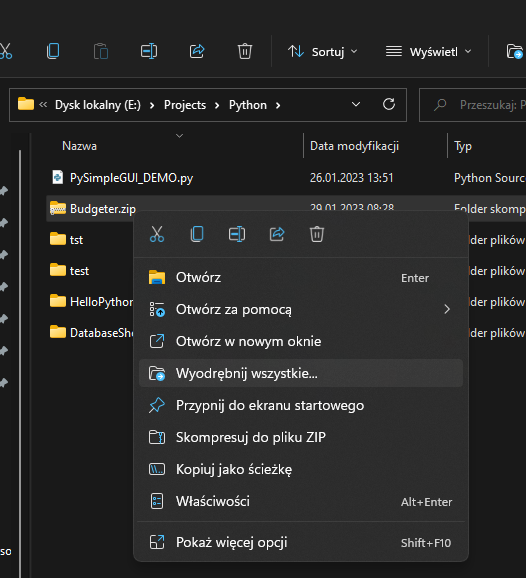
\includegraphics[width=12cm]{figures/Guide/Budgeter_Instruction_01_unzip-archive.png}
\end{figure}

{Po otwarciu archiwum wskaż folder do którego chcesz wypakować aplikację.}

\begin{figure}[H]           %requires float package
    \caption{Wskaż folder}
    \label{fig:Wskaż folder}
    \centering
    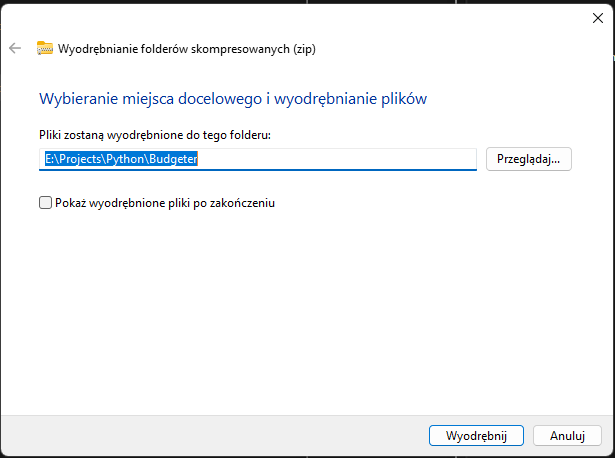
\includegraphics[width=12cm]{figures/Guide/Budgeter_Instruction_01_unzip-archive_p2.png}
\end{figure}

{Po wykakowaniu archiwum w wybranym miejscu pojawi się folder w którym znajduje 
się aplikacja, pozostaje otworzyć ją jak każdy inny program klikając dwukrotnie 
lewym przciskiem myszki i możesz już zacząć swoją przygodę z aplikacją Budgeter.}

\begin{figure}[H]           %requires float package
    \caption{Otwórz katalog}
    \label{fig:Otwórz katalog}
    \centering
    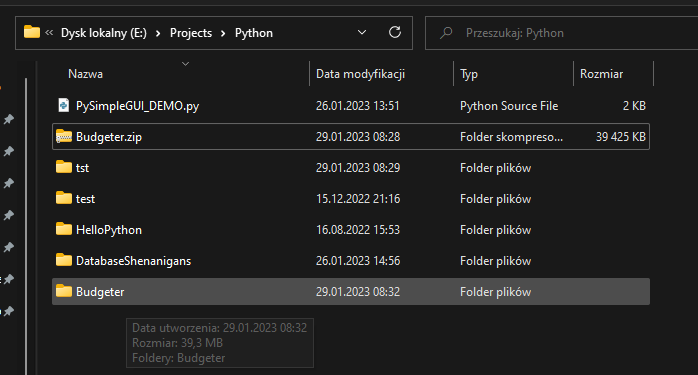
\includegraphics[width=12cm]{figures/Guide/Budgeter_Instruction_02_open.png}
\end{figure}

\begin{figure}[H]           %requires float package
    \caption{Otwóż aplikację}
    \label{fig:Otwóż aplikację}
    \centering
    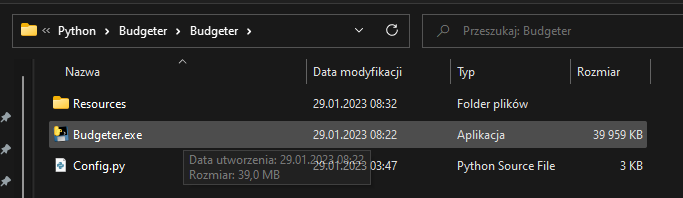
\includegraphics[width=12cm]{figures/Guide/Budgeter_Instruction_02_open_p2.png}
\end{figure}

\begin{figure}[H]           %requires float package
    \caption{Ekran powitalny aplikacji}
    \label{fig:Ekran powitalny aplikacji}
    \centering
    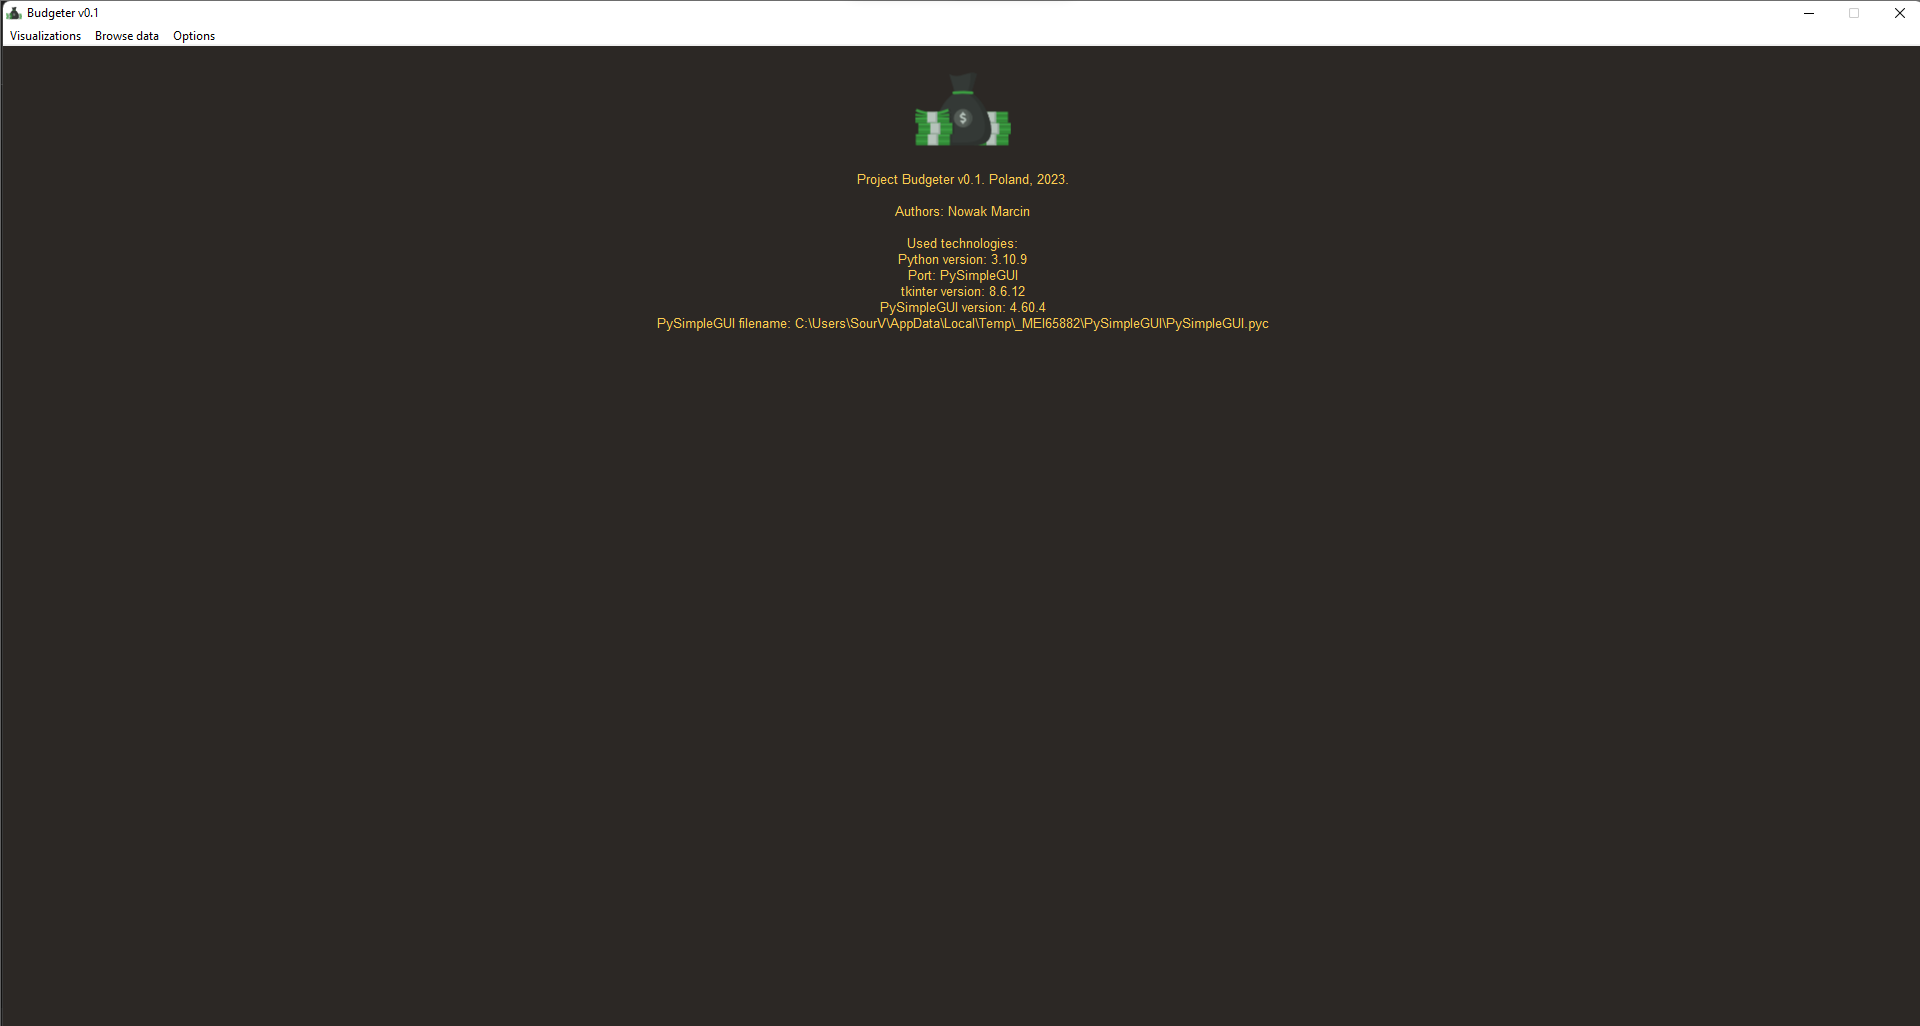
\includegraphics[width=12cm]{figures/Guide/Budgeter_Instruction_03_splashscreen.png}
\end{figure}

\section{\customstylesection{Funkcje i instruykcja obsługi}}
{Przygodę z aplikacją Budgeter warto zacząć od dodania kilku typów produktów, 
w tym celu wejdź w zakładkę Browse Data, następnie wybierz opcję Types.}

\begin{figure}[H]           %requires float package
    \caption{Przeglądanie i edycja danych}
    \label{fig:Przeglądanie i edycja danych}
    \centering
    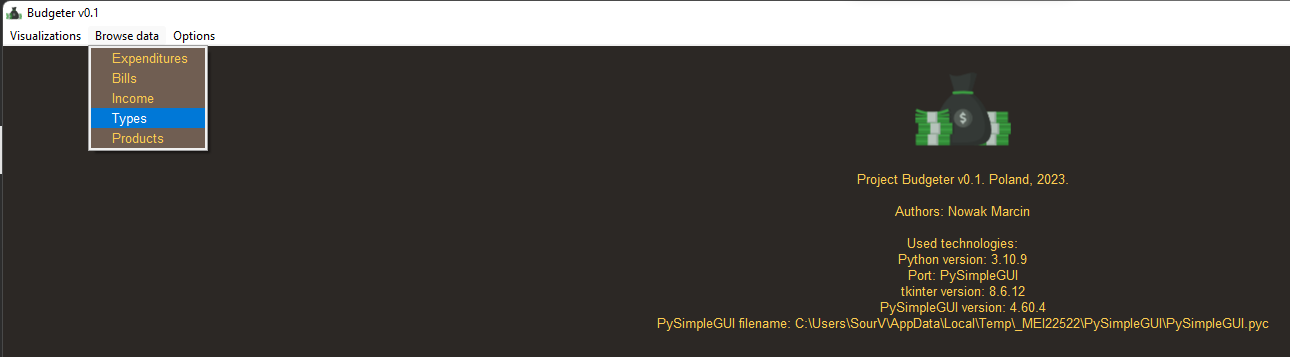
\includegraphics[width=12cm]{figures/Guide/Budgeter_Instruction_04_browse_p1.png}
\end{figure}

{Po otwarciu tabela pokazuje Ci typy które już są w bazie, dodaj swój typ 
naciskając przycisk Add row.}

\begin{figure}[H]           %requires float package
    \caption{Dodawanie rekordu}
    \label{fig:Dodawanie rekordu}
    \centering
    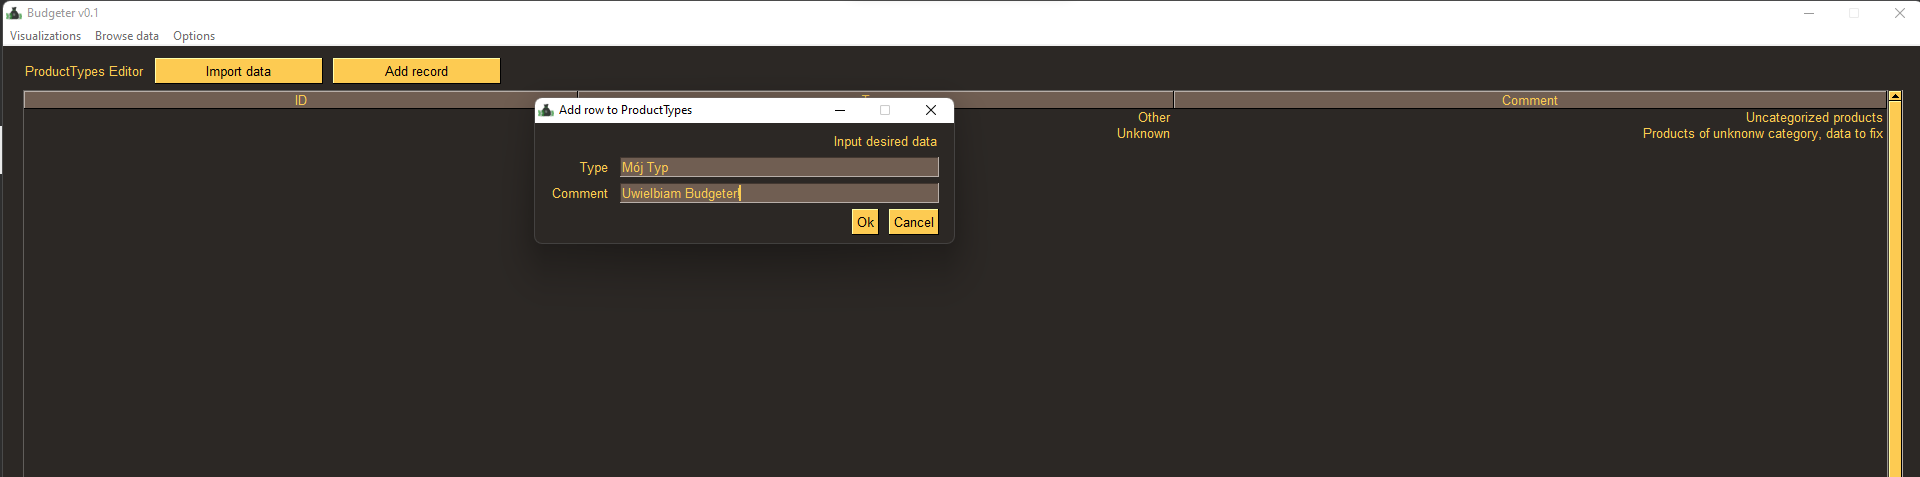
\includegraphics[width=12cm]{figures/Guide/Budgeter_Instruction_04_browse_p2_add_data.png}
\end{figure}

{Dodany rekord pojawia się w wyświetlanej tabeli.}

\begin{figure}[H]           %requires float package
    \caption{Rekord dodany}
    \label{fig:Rekord dodany}
    \centering
    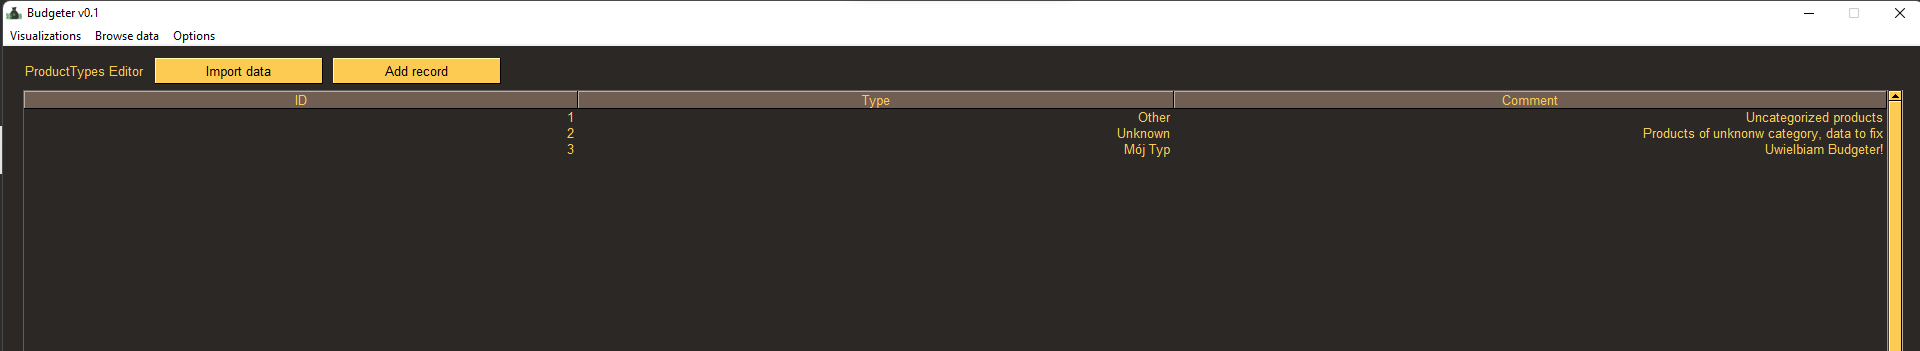
\includegraphics[width=12cm]{figures/Guide/Budgeter_Instruction_04_browse_p3_add_data_success.png}
\end{figure}

{W ten sam sposób dodaj produkty, to pozwoli Ci dodać pierwsze wydatki.}

\medskip
{Wydatki możesz dodać w bardzo podobny sposób, z małymi różnicami. Spójrz na 
poniższą grafikę - pole Products zawiera produkty które zdefiniowałeś w 
poprzednim kroku. Po wypełnieniu wszystkich pól naciśnij przycisk OK a dane 
zostaną zapisane w aplikacji.}

\begin{figure}[H]           %requires float package
    \caption{Dodawanie wydatków}
    \label{fig:Dodawanie wydatków}
    \centering
    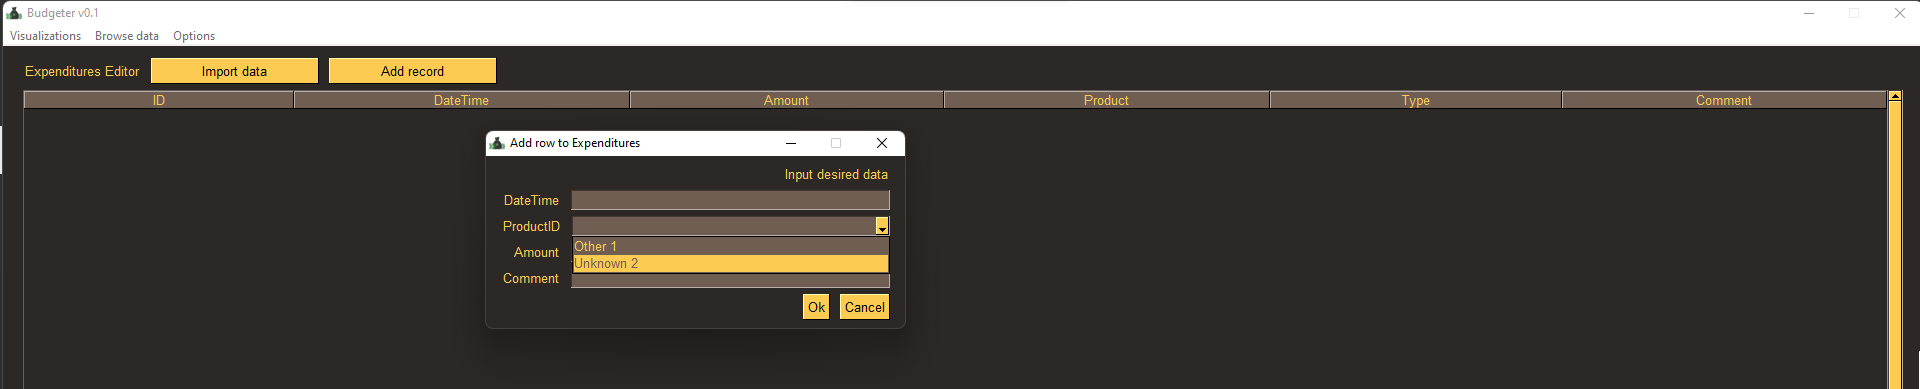
\includegraphics[width=12cm]{figures/Guide/Budgeter_Instruction_04_browse_p4_espenditures.png}
\end{figure}

{Teraz już wiesz jak dodawać dane do wszystkich zbiorów danych. Czasami jednak 
przyda się możliwośc dodania całego zbioru. Dodawanie całego zestawy przez 
wpisywanie każdego rekordu zajmie sporo czasu. Czas jest najcenniejszym z Twoich
 zasobów i Budgeter to szanuje, dlatego możesz także dodać dane importując plik 
w formacie CSV (Comma Separated Values, pliki oddzielane przecinkami). Jeśli 
posiadasz taki plik - a można napisać go ręcznie, wyeksportować z innych 
narzędzi jak chociażby Microsoft Excel - użyj opcji Import data. Pojawi się okno
 wyboru pliku do wczytania, przycisk Browse uruchomi wyszukiwarkę danych. 
Wybierz plik z danymie które chcesz wprowadzić do aplikacji i zatwierdź a dane 
pojawią się w zestawieniu.}

{UWAGA: Uważnie sprawdź czy wybierasz prawidłowy plik, oraz czy dane mają 
kolejność identyczną jak wiodczne w interfejsie. Przez błędne dane aplikacja 
może działać nieprawidłowo.}

\begin{figure}[H]           %requires float package
    \caption{Import danych z pliku}
    \label{fig:Import danych z pliku}
    \centering
    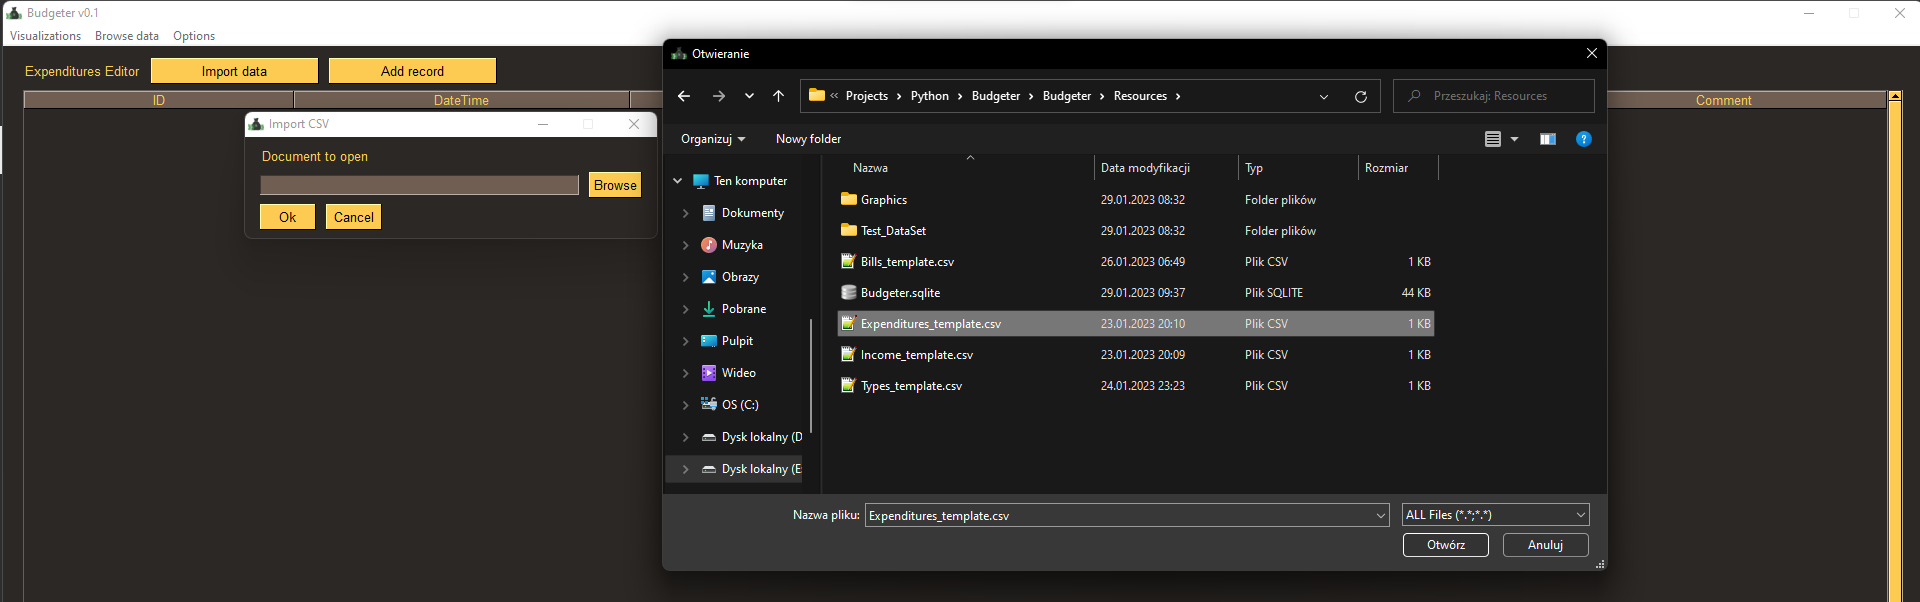
\includegraphics[width=12cm]{figures/Guide/Budgeter_Instruction_05_import-from-csv.png}
\end{figure}

{Teraz pora na najciekawszą funkcję aplikacji - wizualizacje. Dzięki 
wizualizacjom dane wprowadzone do aplikacji zaczynają opowiadać historię. 
Dostęp do nich jest w zasięgu kilku kliknięć myszki - zacznij od zakładki 
Visualizations, po czym wybierz wykres który Cię interesuje a zostanie 
wyświetlony na ekranie.}

\begin{figure}[H]           %requires float package
    \caption{Wizualizacja danych}
    \label{fig:Wizualizacja danych}
    \centering
    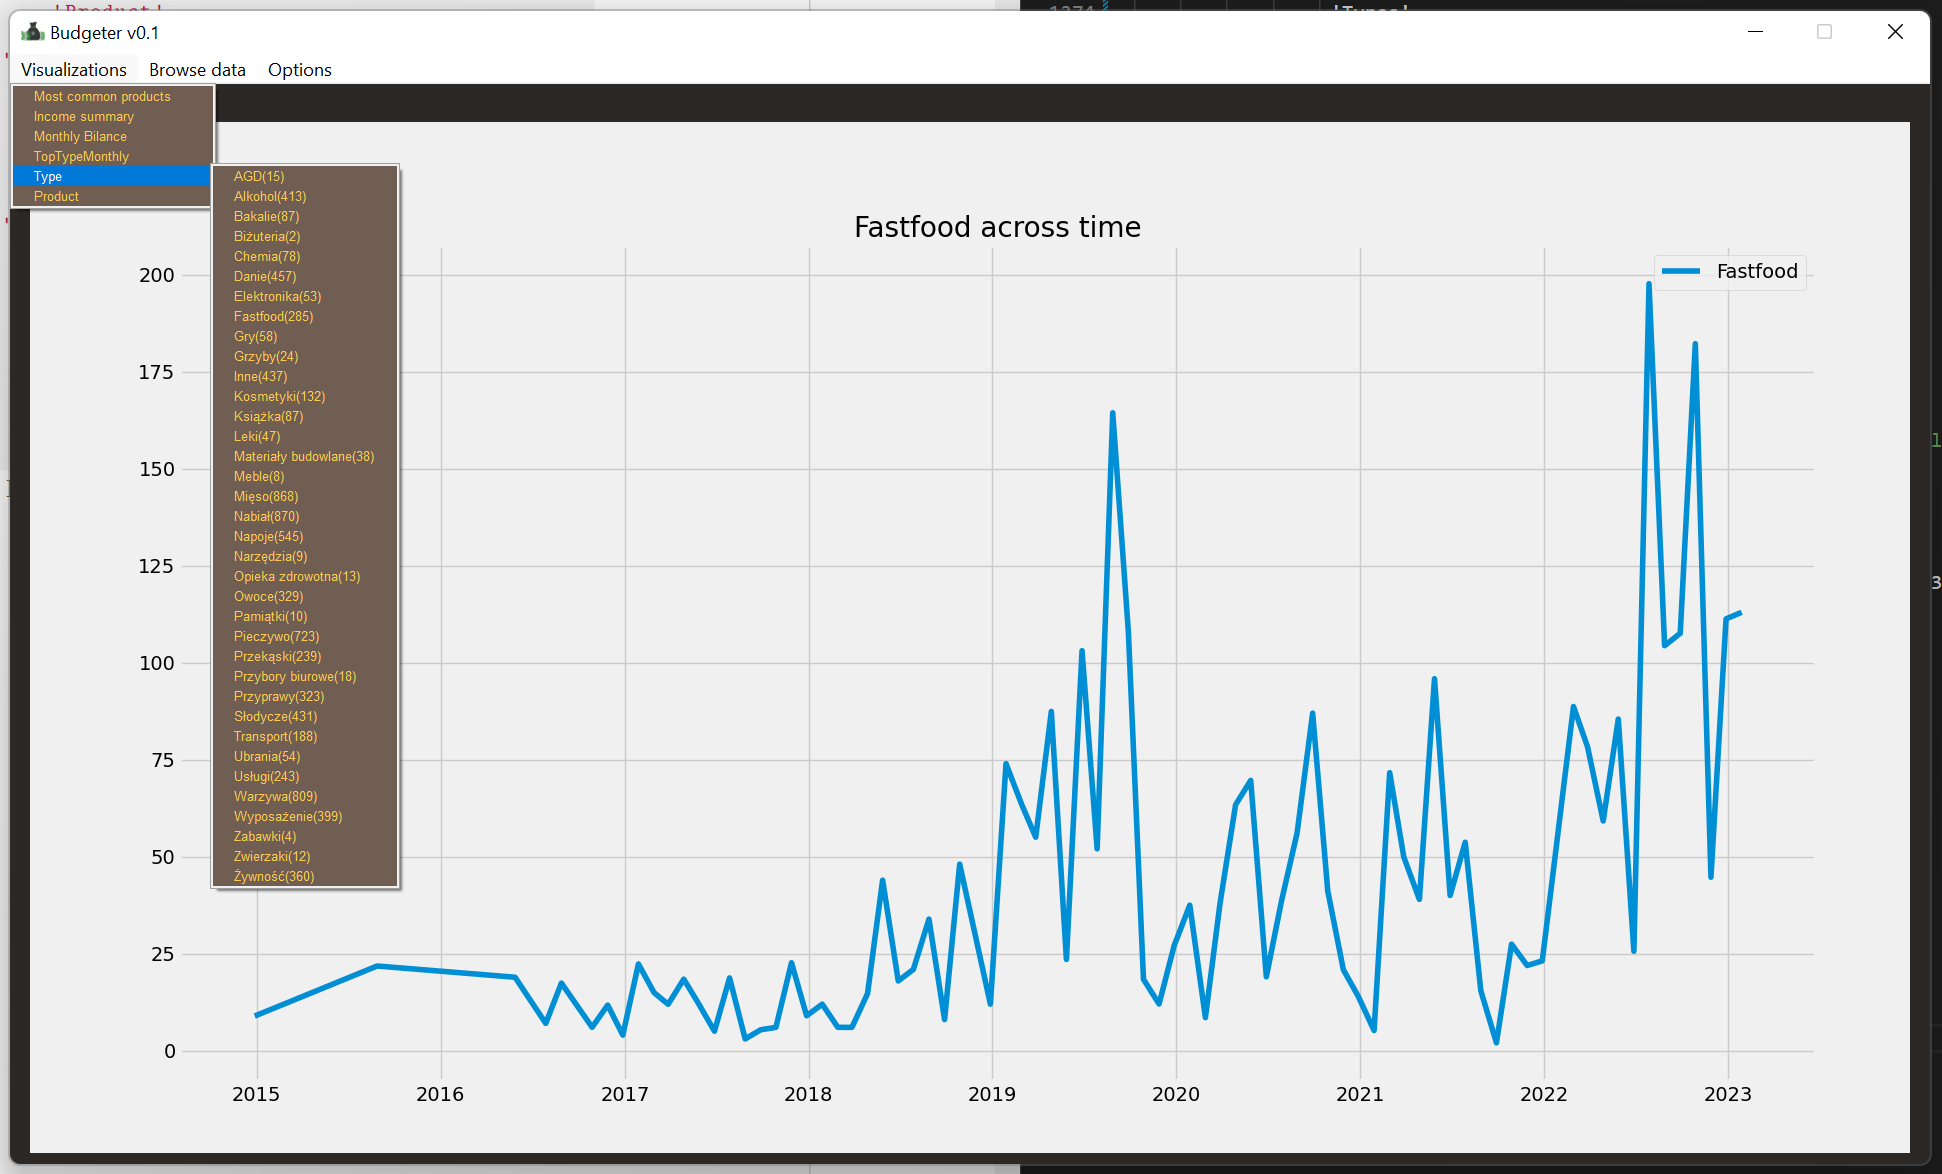
\includegraphics[width=12cm]{figures/Interface_Visualizations_v0.3.png}
\end{figure}

{Do kompletu wiadomości pozostaje już tylko zakładka Options, która zawiera 
dodatkowe, drugorzędne funkcje aplikacji. Opcja About... prezentuje podstawowe 
intformacje o aplikacji i technologiach wykorzystanych w jej wdrożeniu, Manual 
zawierać będzie w przyszłości zintegrowaną instrukję obsługi aplikacji żeby 
wszystkie informacje były zawsze pod ręką. Dzięki opcji Change Team możesz 
dostosować wygląd aplikacji do swoich upodobań.}

\begin{figure}[H]           %requires float package
    \caption{Opcje - zmiana interfejsu}
    \label{fig:Opcje - zmiana interfejsu}
    \centering
    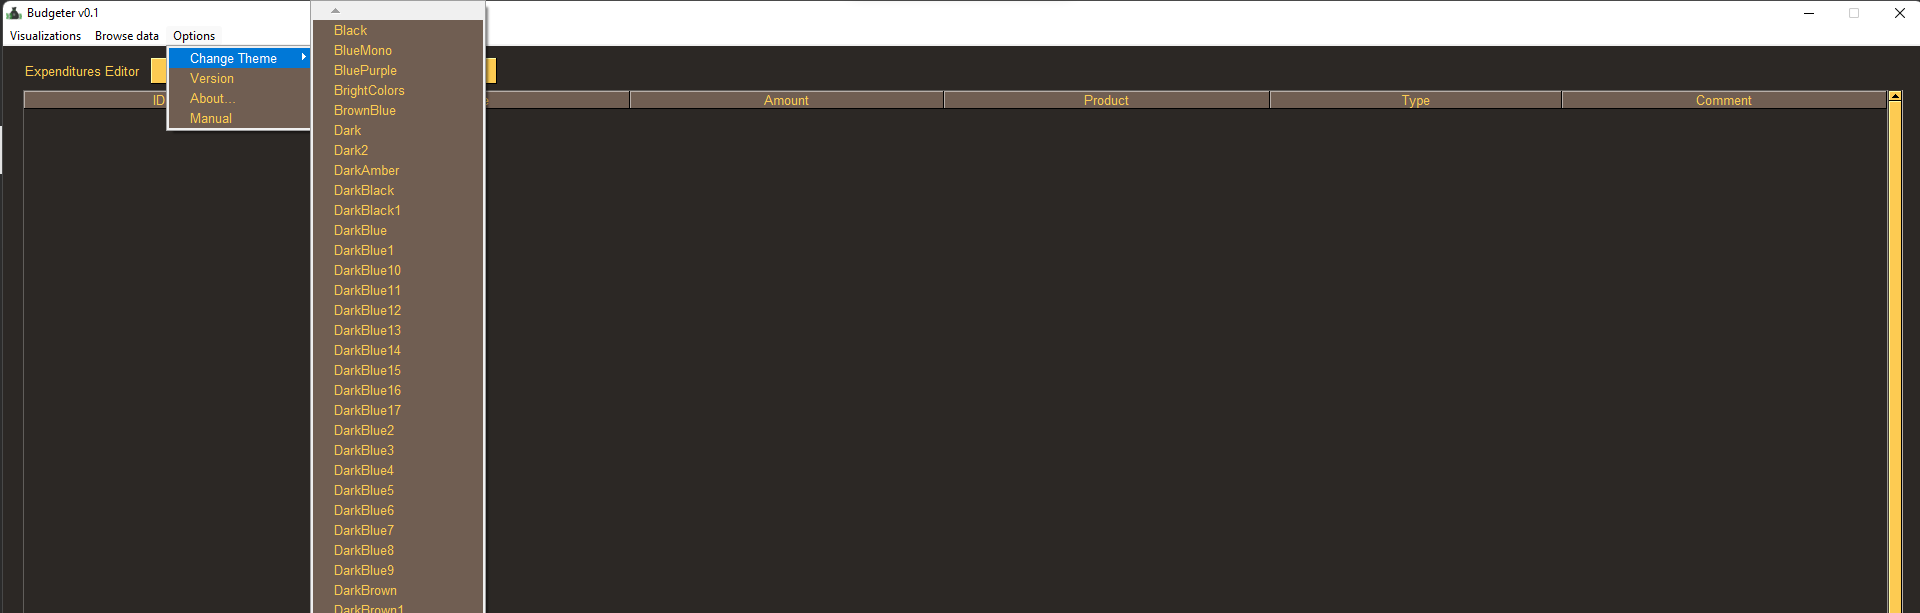
\includegraphics[width=12cm]{figures/Guide/Budgeter_Instruction_06_Options_Change-theme.png}
\end{figure}

\section{\customstylesection{Spostrzeżenia i zalecenia do użytkowania projektu}}
{Obecnie projekt aplikacji Budgeter jest w fazie prototypu, w wyniku tego 
obecnie składa się wyłacznie z głównego modułu analitycznego i wymaganych 
funkcji podstawowych. Drogi użytkowniiku, miej to na uwadze korzystając z 
aplikacji Budgeter - wprowadzaj dane uważnie żeby zapewnić sobie komfort 
korzystania z aplikacji, i rozważ proszę zgłoszenie wszelkich zauważonych 
błędów, co pozwoli dopracować projekt do Twoich oczekiwań. Projekt rozwijany 
będzie na bieżąco dlatego sprawdzaj okresowo czy w repozytorium pojawiła się 
nowa wersja, w ten sposób zyskasz dostęp do nowych funkcji wprowadzonych w 
kolejnych wersjach. Fakt że używasz aplikacji Budgeter oznacza że Twoje dane są 
dla Ciebie ważne, dlatego pamiętaj żeby okresowo zabezpieczać swoje dane żeby 
nie stracić miesięcy wprowadzanych wydatków, przychodów, dopieszczonych 
produktów i ich typów.}

{Przedewszystkim najważniesze zalecenie: czerp przyjemność korzystając z 
aplikacji Budgeter!}

\section{\customstylesection{Potencjalne błędy}}
{Jak każdy program aplikacja Budgeter nie jest wolna od błędów. Należy jednak 
pamiętać że obecnie jest to prototyp, dlatego z pewnością znajdziesz w niej 
wiele możliwych usprawnień warto je zgłosić autorowi projektu, co stwarza szansę
 wyeliminowania błędu w kolejnej wersji oprogramowania.}

{jak wywnioskowałeś z powyższego opisu nie wszystkie błędy są na ten moment 
znane jednak przed kilkoma z nich możesz się ustrzec. Tego typu błędami są:}

\begin{itemize}
    \item Błędne dane wejściowe wpisywane ręcznie - w chwili obecnej aplikacja 
    nie sprawdza całkowicie poprawności danych wejściowych. Wszystkei informacje
     przyjmuje w formie tekstu. W efekcie wprowadzenie błędnych danych 
     najpewniej spowoduje błędne wyświetlanie danych w wykresie.
    \item Błędne dane wejściowe z plikó - jak wyżej
    \item Błędny plik wsadowy - wraz z aplikacją dostarczono szablony plików CSV 
    służących do importu danych do aplikacji. Aplikacja nei sprawdza jednak czy 
    wybrano prawidłowy plik, co pozwala wysłać dane przeznaczone do jednego 
    zbioru (na przykład Produktów) do drugiego, nieprawidłowego (na przykład 
    Wydatków). Aplikacja nie powinna przyjąć takich danych, w tym aspekcie 
    obecnie jest jeszcze rozwijana. Do momentu wydania kolejnej wersji aplikacji
     musisz jednak uważać.
    \item Brak możliwości edycji danych przez aplikację - obecnie nie 
    udostępniamy funkcji edycji danych przez interfejs aplikacji dlatego dbaj 
    o ich prawidłowe wprowadzanie. Użytownicy z dużą wiedzą techniczną wprawnie 
    posługujący się językiem SQL mogą sami połaczyć się z bazą danych aplikacji 
    i poprawić dane bezpośrednio. Jeśłi jednak poprzednie zdanie niewiele Ci 
    mówi warto pozostawić próby poprawy danych do momentu aż taka funkcja pojawi
     się po aktualizacji. 
\end{itemize}


% [REQUIREMENT] 22. Bibliografia - wykaz wszystkich źródeł
\begin{thebibliography} {books}
\bibitem{wiki_ekonomia} Wikipedia, Nauki Ekonomiczne \raggedright\url{
    https://pl.wikipedia.org/wiki/Nauki_ekonomiczne}
\bibitem{gus_sytuacja_budzetowa} Główny Urząd Statystyczny \raggedright\url{
    https://stat.gov.pl/obszary-tematyczne/warunki-zycia/dochody-wydatki-i-warunki-zycia-ludnosci/sytuacja-gospodarstw-domowych-w-2021-r-w-swietle-badania-budzetow-gospodarstw-domowych,3,21.html}
\bibitem{o24_budzetowanie} Opcje24, Budzetowanie \raggedright\url{
    https://www.opcje24h.pl/budzetowanie-przewodnik-planowanie-budzetu/}
\bibitem{MOSCOW} Product Plan, MOSCOW Prioritetization \raggedright\url{
    https://www.productplan.com/glossary/moscow-prioritization/}
\bibitem{MatrycaEisenhowera}Praca.pl, Matryca Eisenhowera - czym jest, zasada, prioryteryzacja zadań \raggedright\url{
    https://www.praca.pl/poradniki/rynek-pracy/matryca-eisenhowera-czym-jest,zasada,prioryteryzacja-zadan_pr-2012.html}
\bibitem{MVP} Wikipedia, Minimal Viable Product \raggedright\url{
    https://en.wikipedia.org/wiki/Minimum_viable_product}
\bibitem{ISO 8601} NASA.gov, A summary of the international standard date and time notation \raggedright\url{
    https://fits.gsfc.nasa.gov/iso-time.html}
\bibitem{CSV} Y. Shafranovich, SolidMatrix Technologies, Inc., Common Format and MIME Type for Comma-Separated Values (CSV) Files \raggedright\url{
    https://www.rfc-editor.org/rfc/rfc4180}
\bibitem{SQLite} sqlite.org, SQLite \raggedright\url{
    https://www.sqlite.org/index.html}
\bibitem{SQL} wikipedia.org, SQL - Structured Query Language \raggedright\url{
    https://en.wikipedia.org/wiki/SQL}
\bibitem{Python} python.org, Python \raggedright\url{
    https://www.python.org/}
\bibitem{PySimpleGUI} pysimplegui.org, PySimpleGUI Python GUIs for Humans \raggedright\url{
    https://www.pysimplegui.org/en/latest/}
\bibitem{JSON} json.org, Introducing JSON \raggedright\url{
    https://www.json.org/json-en.html}
\bibitem{Python_read-file} pythonspot.com, Python tutorials, How to Read a File in Python \raggedright\url{
    https://pythonspot.com/read-file/}
\bibitem{Trello} Atlassian, Trello.com \raggedright\url{
    https://trello.com/}
\bibitem{StarUML} MKLabs Co.,Ltd, StarUML \raggedright\url{
    https://staruml.io/}
\bibitem{LaTeX} The LaTeX Project \raggedright\url{
    https://www.latex-project.org/}
\bibitem{VSCode} Microsoft, Visual Studio Code \raggedright\url{
    https://code.visualstudio.com/}
\bibitem{DataGrid} JetBrains, DataGrid \raggedright\url{
    https://www.jetbrains.com/datagrip/}
\bibitem{Kanban} Lean Action PLan, Kanban – układ nerwowy sterowania produkcją w koncepcji Lean Manufacturing \raggedright\url{
    https://leanactionplan.pl/kanban/}
\bibitem{LEAN} Wikipedia, Lean software development \raggedright\url{
    https://pl.wikipedia.org/wiki/Lean_software_development}
\bibitem{GIT} git-scm.com, git \raggedright\url{
    https://git-scm.com/}
\bibitem{GitHub} https://github.com/ \raggedright\url{
    https://github.com/}
\bibitem{Model Przyrostowy} Wikipedia, Model Przyrostowy \raggedright\url{
    https://pl.wikipedia.org/wiki/Model_przyrostowy}
\bibitem{EdittableTable} YouTube The CS Classroom, PySimpleGUI - Excel-style Editable Table \raggedright\url{
    https://www.youtube.com/watch?v=ETHtvd-_FJg}
\bibitem{Tkinter} python.org, tkinter — Python interface to Tcl/Tk \raggedright\url{
    https://docs.python.org/3/library/tkinter.html}
\bibitem{PyInstaller} pyinstaller.org, PyInstaller Manual \raggedright\url{
    https://pyinstaller.org/en/stable/}
\bibitem{GITBudgeterApp} github.com MarcinNowak94, DatabaseShenanigans \raggedright\url{
    https://github.com/MarcinNowak94/DatabaseShenanigans}
\bibitem{GITBudgeterDoc} github.com MarcinNowak94, budgeter \raggedright\url{
    https://github.com/MarcinNowak94/budgeter}

\end{thebibliography}

% [REQUIREMENT] 21. Spisy ilustracji (spis obiektów graficznych, diagramów, tabel...)
\listoffigures
\listoftables
\lstlistoflistings

\end{document}


% ------------------------------ Docummentation -------------------------------
% [REQUIREMENT] 1. Strona tytułowa
% [REQUIREMENT] 2. Spis treści
% [REQUIREMENT] 3. Wprowadzenie do tematyki projektu
% [REQUIREMENT] 4. Zamierzony cel projektu
% [REQUIREMENT] 5. Wstępne założenia i uwarunkowania, w których 
% projekt będzie powstawał  -----------------------
% [REQUIREMENT] 6. Założone ograniczenia (ramy czasowe, umiejętności) 
% i możliwość ewaluacji projektu
% [REQUIREMENT] 7. Chronologiczny plan pracy (ujecie przyjetego modelu 
% projektowania i faz projektowania)
% [REQUIREMENT] 8. POWYŻSZĄ CZĘŚĆ DOKUMENTACJI ODDAJEMY PRZED REALIZACJĄ PROJEKTU
% [REQUIREMENT] 9. Wymagania funkcjonalne (szczegółowey wykaz wszystkich funkcji 
% oprogramowania) jakie funkcjonalności oprogramowania chcemy dostarczyć, można 
% nie zdążyć z dostarczeniem części, lub dopisać dodatkowe dodane w trakcie
% [REQUIREMENT] 10. Wymagania niefunkcjonalne
% [REQUIREMENT] 10.1. Sprzętowe (w różnych wariantach, w tym dostęp do 
% koniecznych lub alternatywnych nośników danych i peryferiów)
% [REQUIREMENT] 10.2. Systemowe (systemy operacyjne, zainstalowane środowiska, 
% platformy, pakiety, biblioteki, sterowniki)
% [REQUIREMENT] 10.3. Organizacyjne (np. organizacja pracy z systemem, warunki 
% poprawnej pracy przy większej liczbie użytkownikó, stanowisk, obciążeniu sieci,
% konieczność zapewnienia realnego czasu dostępu itd.itp.)
% [REQUIREMENT] 11. Wymagania dotyczące danych (wykaz tabel, relacji, 
% typy i rozmiary pól z uzasadnieniem, inne rodzaje danych w tym logi, hasła)
% [REQUIREMENT] 12. Metody pracy, narzędzia i techniki
% [REQUIREMENT] 13. Opis głównych klas, metod, obiektów, struktur i algorytmów
% zastosowanych w projekcie (uwzględniając stsosowanie gotowych narzędzi
% obcego autorstwa, w tym open source)
% [REQUIREMENT] 14. POWYŻSZĄ CZĘŚĆ DOKUMENTACJI ODDAJEMY W TRAKCIE TWORZENIA
% [REQUIREMENT] 15. Przebieg uruchamiania projektu (być może na różnych 
% platformach, konfiguracjach...)
% [REQUIREMENT] 16. Przebieg testowania projektu (rodzaje i metody przeprowadzonych
% testów)
% [REQUIREMENT] 17. Wnioski z przebiegu testowania (wykryte defekty, wrażliwość
% na specyficzne dane, błędy ukryte i niewidoczne dla użytkownika, sytuacje
% niejednoznaczne itp.)
% [REQUIREMENT] 18. Konserwacja systemu
% [REQUIREMENT] 19. Podsumowanie i alternatywne sposoby stworzenia projektu
% (po zdobytym doświadczeniu, przy dostępie do innych narzędzi, przy innej wizji...)
% [REQUIREMENT] 20. Dokumentacja dla użytkownika (Podręczni kużytkownika)
% [REQUIREMENT] 20.1. Przeznaczenie i główne możliwości systemu
% [REQUIREMENT] 20.2. Podstawowe wymagania
% [REQUIREMENT] 20.3. Opis instalacji/uruchamiania
% [REQUIREMENT] 20.4. Kompletny opis działających funkcji (menu, opis interface...),
% formatów danych, obsługi błędów użytkowania, zakresów danych 
% [REQUIREMENT] 20.5. Podręcznik administratora/użytkownika systemu/gościa
% [REQUIREMENT] 20.6. Spostrzeżenia i zalecenia do użytkowania projektu
% [REQUIREMENT] 20.7. Wykryte błędy w działaniu
% [REQUIREMENT] 21. Spisy ilustracji (spis obiektów graficznych, diagramów, tabel...)
% [REQUIREMENT] 22. Bibliografia - wykaz wszystkich źródeł
% [REQUIREMENT] 23. Przypisy dolne, stopki (nr stron), nagłówki...

% --------------------------------- Purgatory ----------------------------------
% Orphaned snippets of texts placed here untill you decide what to do with them
% -----
% domowym i udostępnienie podstawowych informacji finansowych Niestety jedak 
% zakres wiedzy w zakresie finansów którą posiada przeciętny obywatel jest dość 
% niski, w połączeniu z obecnie panującą trudną sytuacją gospodarczą w wielu 
% miejscach na świecie część ludzi nie radzi sobie z dopinaniem budżetu 
% domowego. Jest to jednak dziedzina dość skomplikowana, a tym samym trudna dla 
% przeciętnego obywatela.